\chapter{Digital Model for Elastica}
\label{chapter:digital-model-elastica}

In this chapter we review the elastica energy and some of its properties. Next, we introduce the digital version of the elastica using multigrind convergent estimators of length and curvature. Finally, we describe a theoretical optimization model for the minimization of the digital elastica.

\section{Continuous and Digital Elastica}
	\sketch{To be developed...}
	
	
	Given an Euclidean shape $X$, its digital elastica $\hat{E}$ is defined as
	\begin{align}
	\hat{E}( D_h(X) ) = \sum_{\dot{\vec{e}} \in \partial D_h(X)}{ \hat{s}( \dot{\vec{e}})\left(\; \alpha + \beta \hat{\kappa}_{r}^2(D_h(X),\dot{\vec{e}},h) \; \right)},
	\label{eq:digital-elastica}
	\end{align}
	
where $\dot{\vec{e}}$ denotes the center of the edge $\vec{e}$. In the
expression above, we will substitute an arbitrary subset $Z$ of
$\mathbb{Z}^2$ to $D_h(X)$ since the continuous shape $X$ is unknown.
In the following we omit the grid step $h$ to simplify expressions
(or, putting it differently, we assume that the shape of interest is
rescaled by $1/h$ and we set $h=1$). 

In the next section, we describe a combinatorial scheme that permit us to find the minimum digital shape with respect the digital elastica energy for some neighborhood of shapes of $S$. 

\section{Local Combinatorial Scheme}

Given a digital shape $S^{(0)}$ we describe a process that generates a
sequence $S^{(i)}$ of shapes with non-increasing Elastica energy. The
idea is to define a neighborhood of shapes $\mathcal{N}^{(i)}$ to the
shape $S^{(i)}$ and choose the element of $\mathcal{N}^{(i)}$ with
lowest energy.  The process is suited for the integral invariant
estimator but also for other curvature estimators, for example, MDCA
\cite{roussillon11mdca}. As a matter of fact, our experiments have
shown that either estimators induce similar results.

Let $S \subset \Omega$ be a $2$-dimensional digital shape. We adopt the cellular-grid model to represent $S$, i.e., pixels and its lower dimensional counterparts, linels and pointels, are part of $S$. In particular, we denote by $\partial S$ the topological boundary of $S$, i.e., the connected sequence of linels such that for each linel we have one of its incident pixels in $S$ and the other not in $S$.


Let $d_{S}:\Omega \rightarrow \mathcal{R}$ be the signed Euclidean distance transformation with respect to shape $S$. The value $d_S(x)$ gives the Euclidean distance between $x$ and the closest linel in $\partial S$. 

\begin{definition}{m-Ring Set}
Given a digital shape $S\in\Omega$, its distance transformation $d_S$ and natural number $m > 0$, the {\em $m$-ring set of $S$} is defined as
\begin{align*}
	\quad R_m(S) &:= R_m^-(S) \; \cup \; R_m^+(S) \\
	&:= \left\{ x \in \Omega \; | \; -m \leq d_S(x) < -(m-1) \right\} \; \cup \;  \left\{ x \in \Omega \; | \; 	m-1 < d_{S}(x) \leq m \right\}.
\end{align*}
\end{definition}

Consider the following set of neighbor candidates to $S$ using the $1-Ring$ os $S$:
\begin{align*}
\mathcal{U}(S) = \{ D \; | D \subset R_1(S) \cup S \; \text{and} \; \text{$D$ is connected} \}.
\end{align*}


A shape with $n$ linels in its topological boundary has a neighborhood size of order $O(2^n)$, and its complete exhaustion is inconceivable.  Instead, we explore a subset of it with the help of $n$-glued curves.

An oriented closed curve $C$ is a closed connected sequence of linels with a well-defined interior. A segment of $C$ is a connected subsequence $c \in C$ of its linels.


\begin{definition}{Glued Curve}
Given closed curves $C_1,C_2$ agreeing with some orientation $q$, a glued curve is a closed curve  $(c_1,\ell_1,c_2,\ell_2)$ with orientation $q$ and $c_1 \in C_1, c_2 \in C_2$. The linels $\ell_1,\ell_2$ are called junction linels.
\end{definition}

\begin{definition}{$n$-Glued Curve Set}
Given closed curves $C_1,C_2$ with same orientation, its set of $n$-glued curves is defined as
\begin{align*}
	\mathcal{G}_n(C_1,C_2) = \{ (c_1,\ell_1,c_2,\ell_2) \; | \; |c_2|=n \},
\end{align*}
\end{definition}

Let $S_O = ( S \cup R_1^+(S) ) $ and $S_I = ( S \setminus R_1^-(S) ) $, the neighborhood set to shape $S$ is defined as
\begin{align*}
	\mathcal{N}(S,N) = \bigcup_{1 \leq n \leq N} int \big( \mathcal{G}_{n}(\partial S_O, \partial S) \; \big) \cup int \big( \;  \; \mathcal{G}_{n}(\partial S, \partial S_I) \; \big),
\end{align*}

where $int(C)$ is the interior of the shape bounded by the closed oriented curve $C$. Algorithm~\ref{alg:local-search} describes the local combinatorial process and Figure~\ref{fig:local-comb-square-results} presents the digital curve evolution when executing this algorithm for several shapes with $N=50$.


\begin{figure}[h!]
\center
\subfloat{
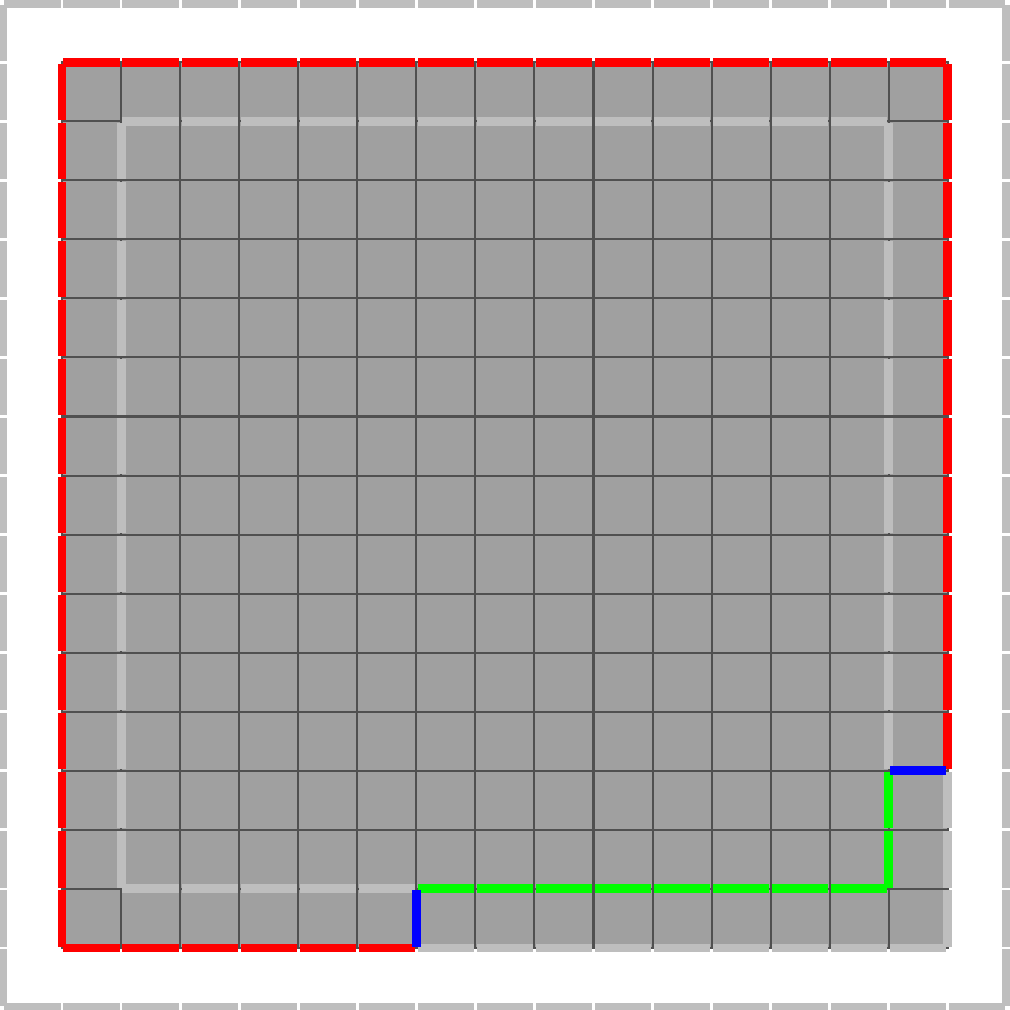
\includegraphics[scale=0.4]{figures/chapter5/gcurves/main-inner.pdf}
}\hspace{1em}%
\subfloat{
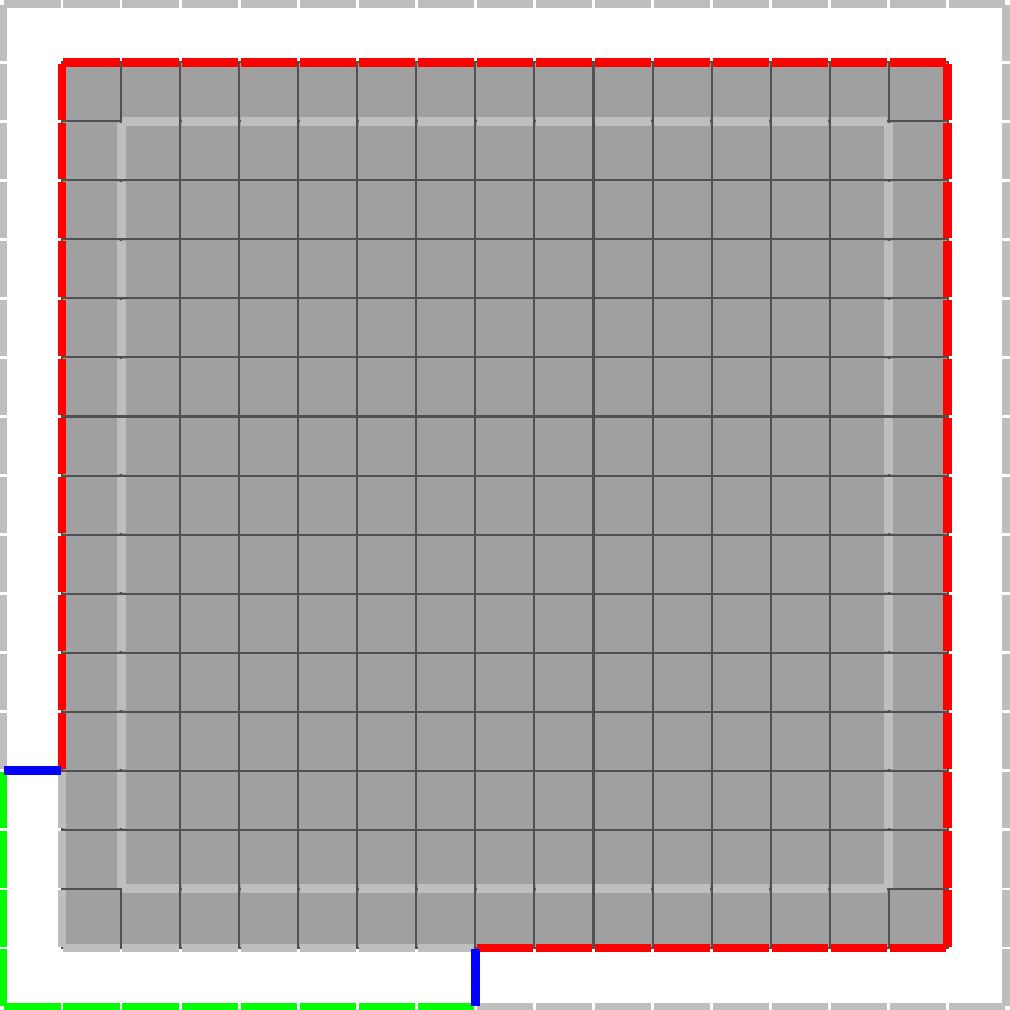
\includegraphics[scale=0.4]{figures/chapter5/gcurves/main-outer.pdf}
}\hspace{1em}\\[1em]
\subfloat{
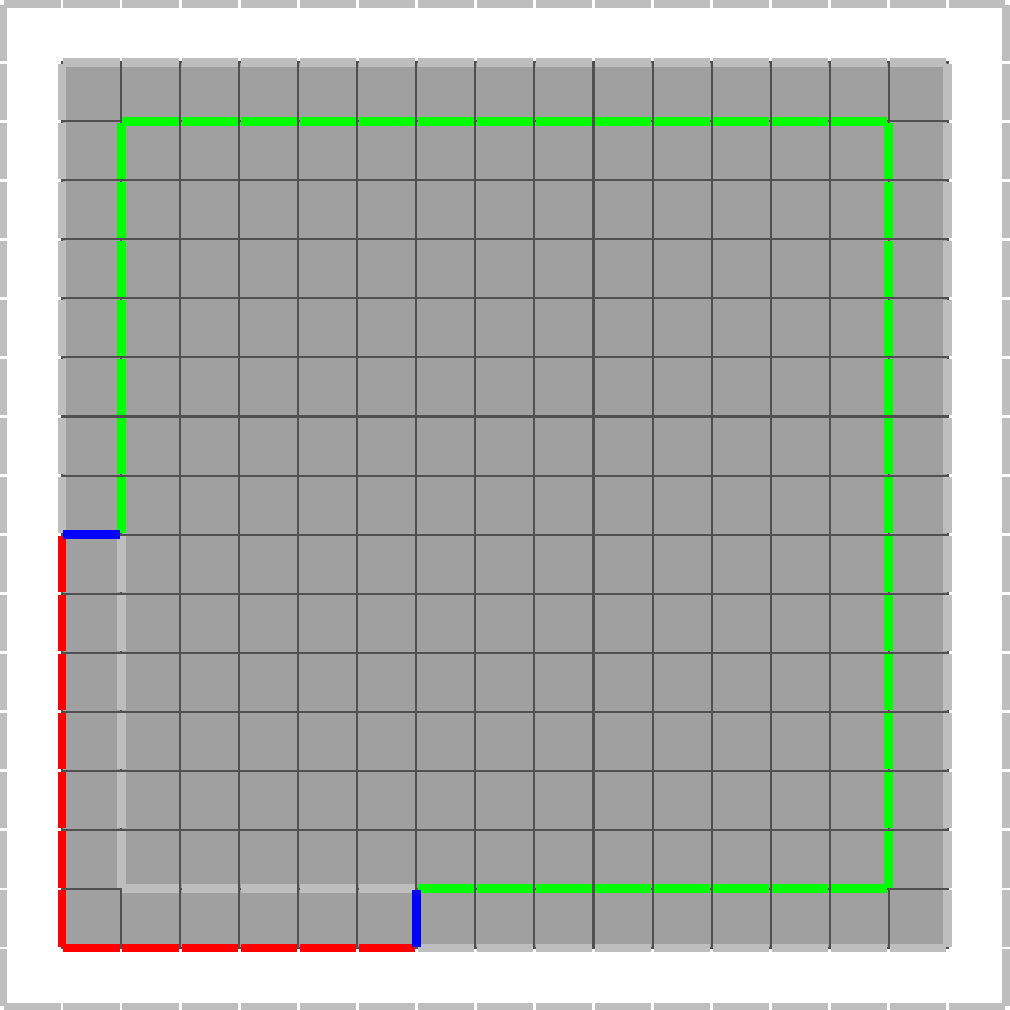
\includegraphics[scale=0.4]{figures/chapter5/gcurves/inner-main.pdf}
}\hspace{1em}%
\subfloat{
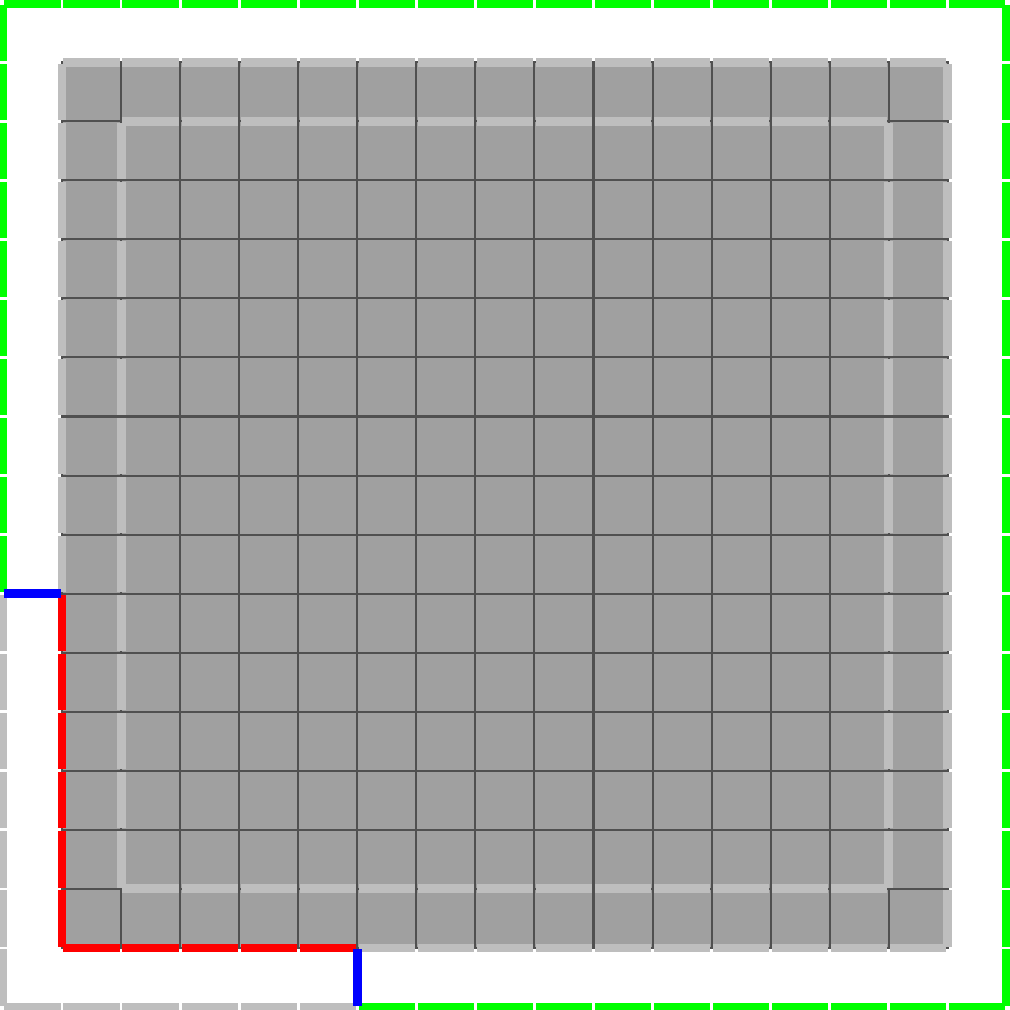
\includegraphics[scale=0.4]{figures/chapter5/gcurves/outer-main.pdf}
}\hspace{1em}%
\caption{Examples of $10$-Glued curves.}
\end{figure}


\begin{algorithm}[H]
 \SetKwData{It}{i}
 \SetKwData{MIt}{maxIt}
 \SetKwData{Tol}{tolerance}
 \SetKwData{Delta}{delta}
 \SetKwData{Best}{best} 
 \SetKwInOut{Input}{input}\SetKwInOut{Output}{output}
 
 \Input{A digital set $S$; the maximum length of glued curves $N$; the maximum number of iterations \MIt; and a stop condition \Tol}
 \BlankLine
 \Delta $\longleftarrow$ \Tol+1\;
 \While{ \It $<$ \MIt \bf{and} \Delta $>$ \Tol  }{
  	\For{$ X \in \mathcal{N}(S^{(i)},N) $}
	{
		\If{ $\hat{E}(X)$ $<$ $\hat{E}(X^\star)$ }
		{
			$X^\star \longleftarrow X$
		}
	}
	\It $\longleftarrow$ \It $+1$\;
	$S^{(i)} \longleftarrow X^\star$\;
	\Delta $\longleftarrow$ $\hat{E}(S^{(i-1)}) - \hat{E}(S^{(i)})$\;	
 }
 \label{alg:local-search} 
 \caption{Local combinatorial optimization for elastica minimization.}
\end{algorithm}

\begin{figure}[h!]
\center
\subfloat{
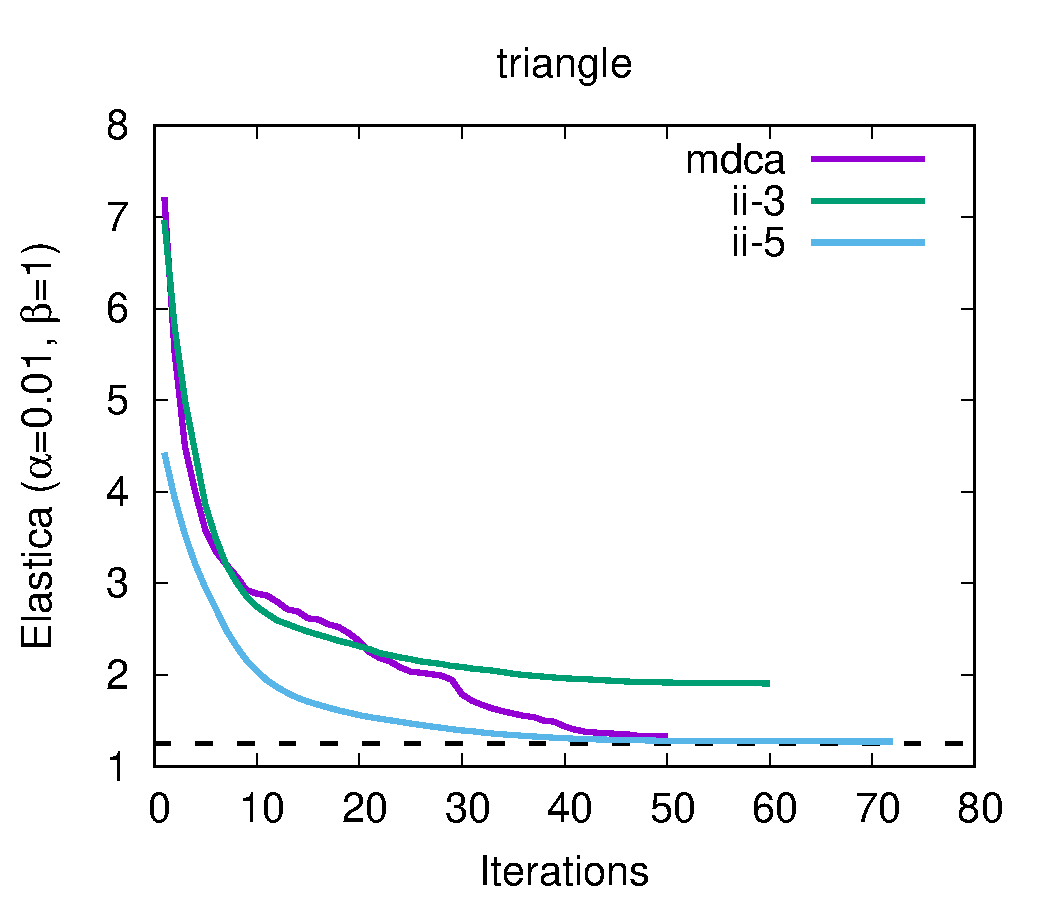
\includegraphics[scale=0.4]{figures/chapter5/exhaustive-selection/plot-shape-estimator/triangle.pdf}
}\hspace{1em}%
\subfloat{
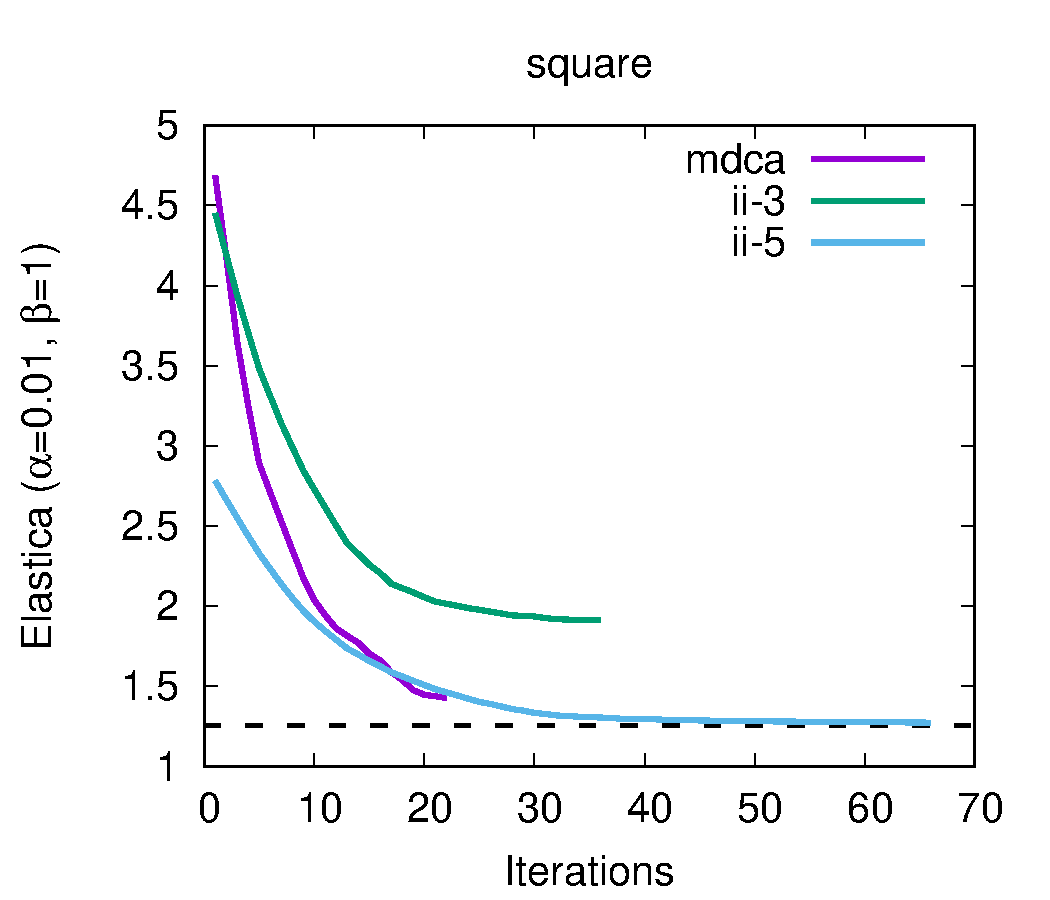
\includegraphics[scale=0.4]{figures/chapter5/exhaustive-selection/plot-shape-estimator/square.pdf}
}\hspace{1em}%
\subfloat{
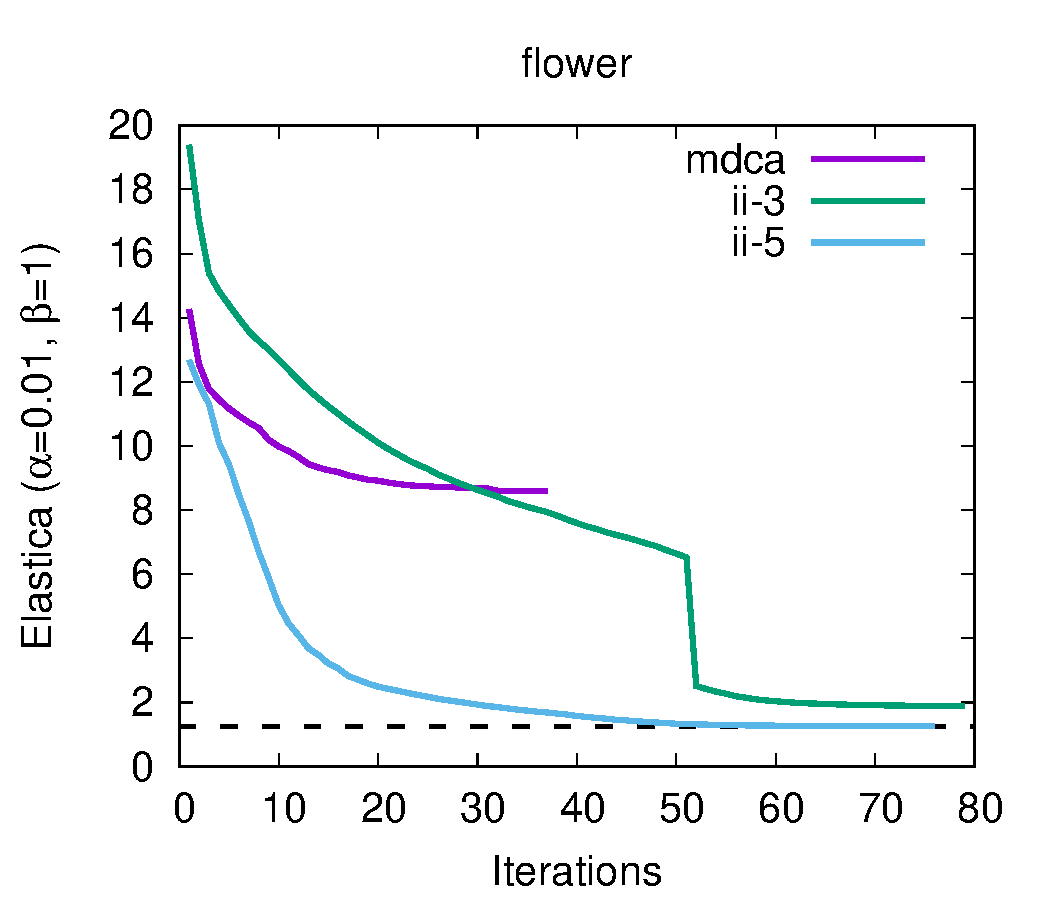
\includegraphics[scale=0.4]{figures/chapter5/exhaustive-selection/plot-shape-estimator/flower.pdf}
}\hspace{1em}%
\subfloat{
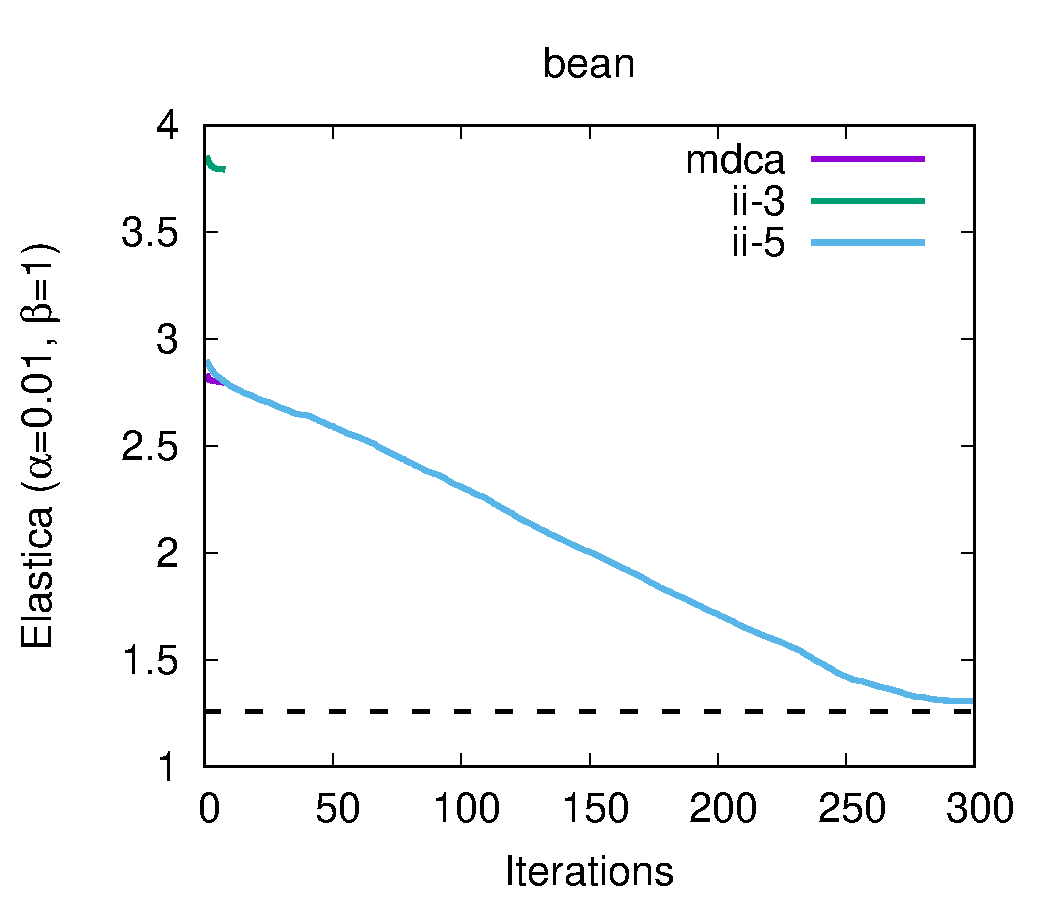
\includegraphics[scale=0.4]{figures/chapter5/exhaustive-selection/plot-shape-estimator/bean.pdf}
}%
\caption{Elastica value evolution for the triangle, square, flower and bean shapes. Evolution with II-$5$ estimator achieves global optima (dashed line) for the first three shapes.}
\label{fig:local-comb-plots}
\end{figure}

\begin{figure}[!h]
\center
\begin{minipage}[b]{0.5\textwidth}
\center
	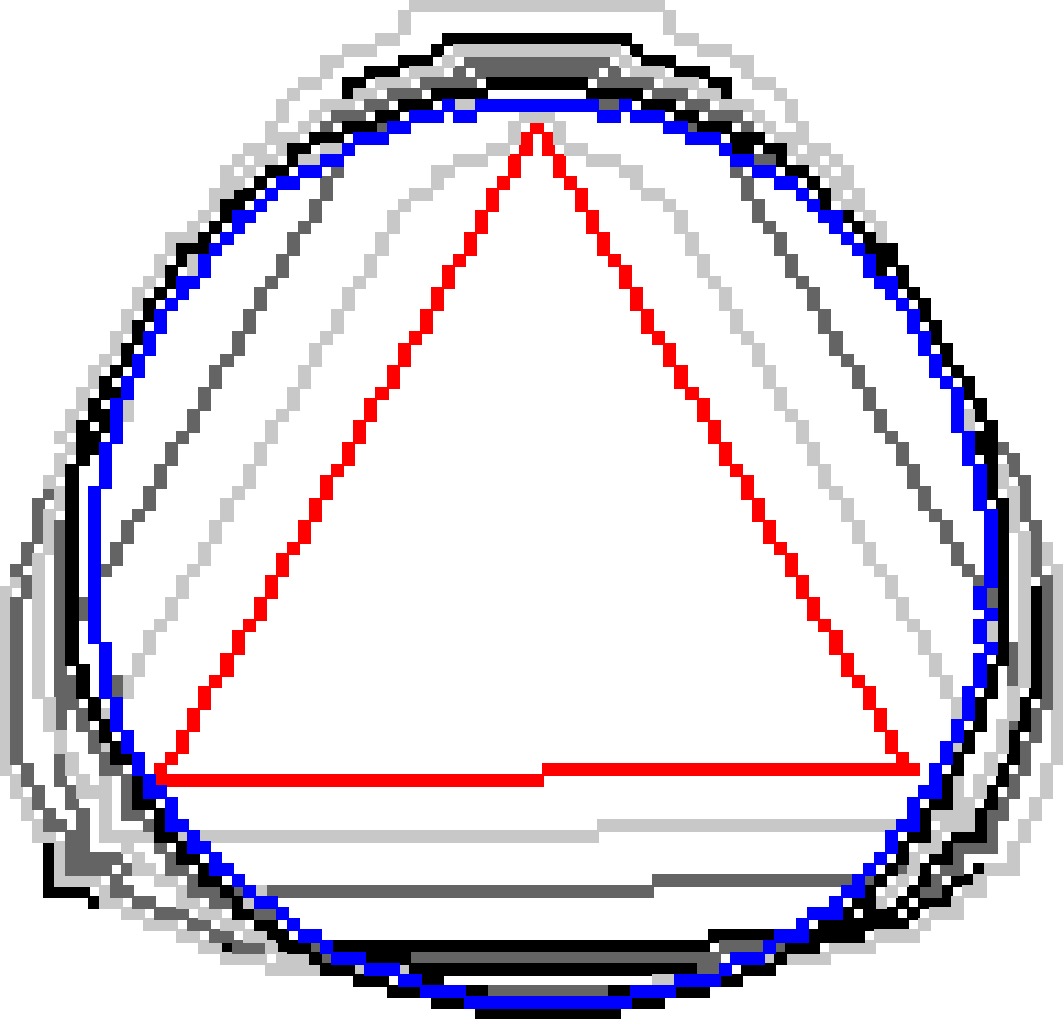
\includegraphics[scale=0.185]{figures/chapter5/exhaustive-selection/ii-r5-lp0.01/triangle/summary.pdf}\\[2em]
	
	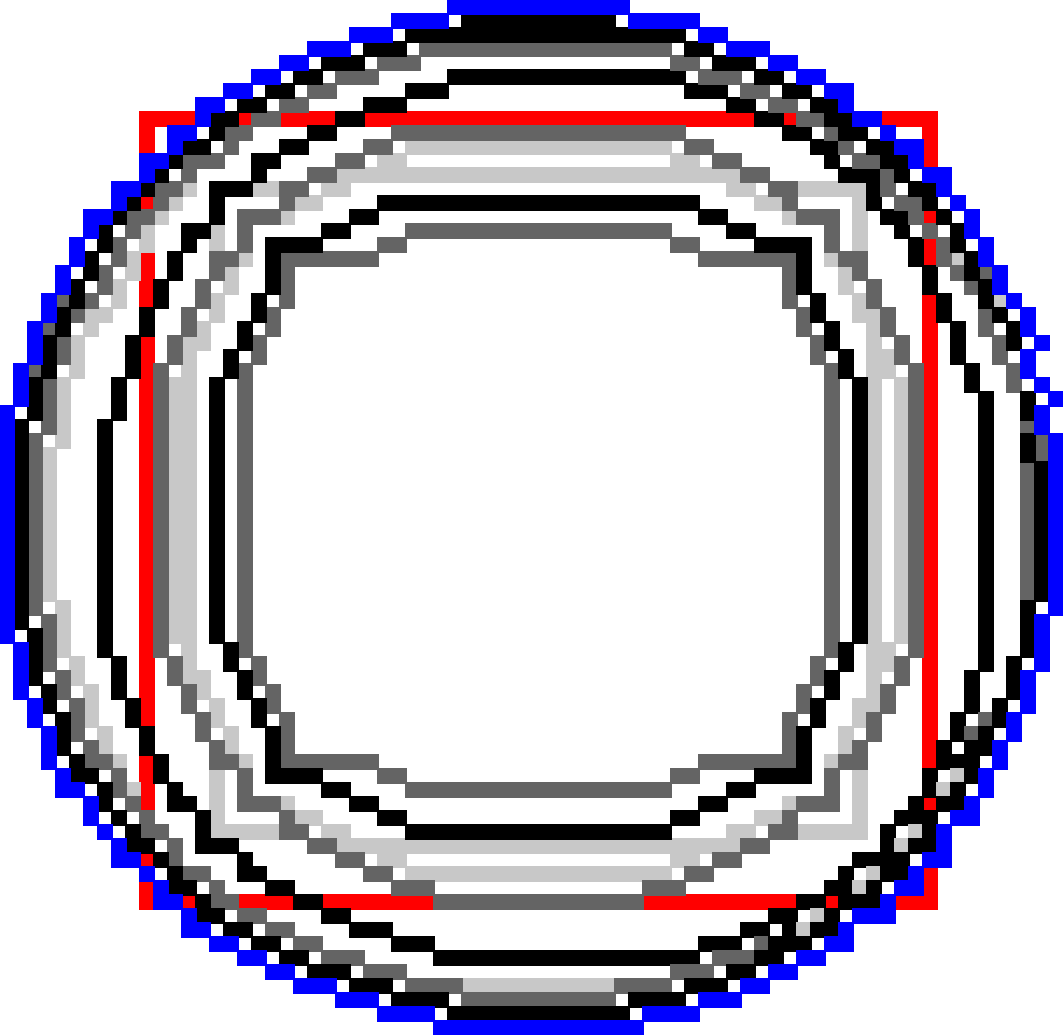
\includegraphics[scale=0.17]{figures/chapter5/exhaustive-selection/ii-r5-lp0.01/square/summary.pdf}\\[2em]

	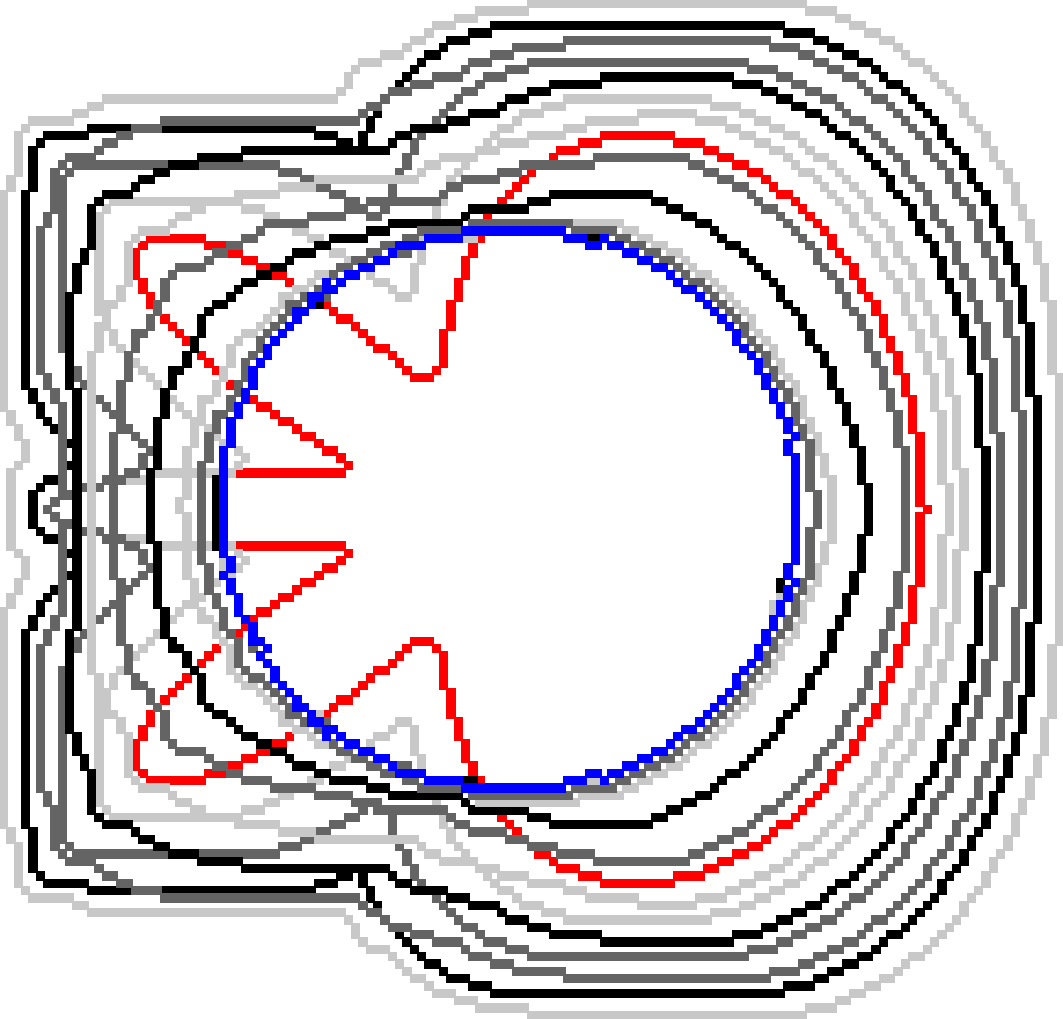
\includegraphics[scale=0.25]{figures/chapter5/exhaustive-selection/ii-r5-lp0.01/flower/summary.pdf}\\[2em]		
	
	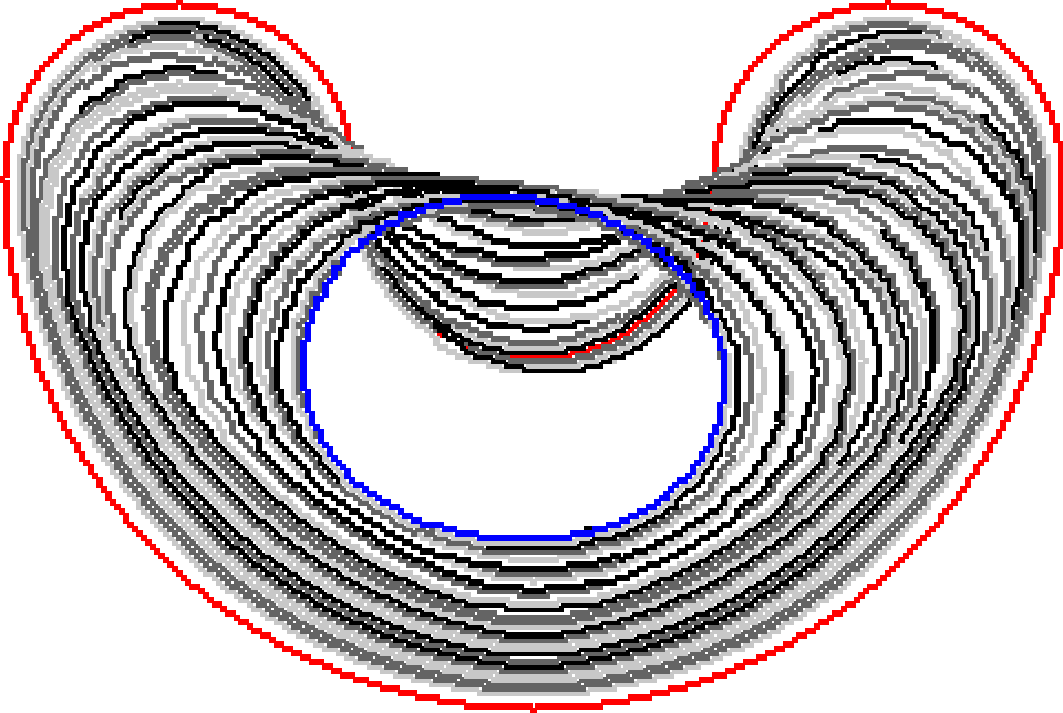
\includegraphics[scale=0.25]{figures/chapter5/exhaustive-selection/ii-r5-lp0.01/bean/summary.pdf}			
\end{minipage}%
\begin{minipage}[b]{0.5\textwidth}
\center
	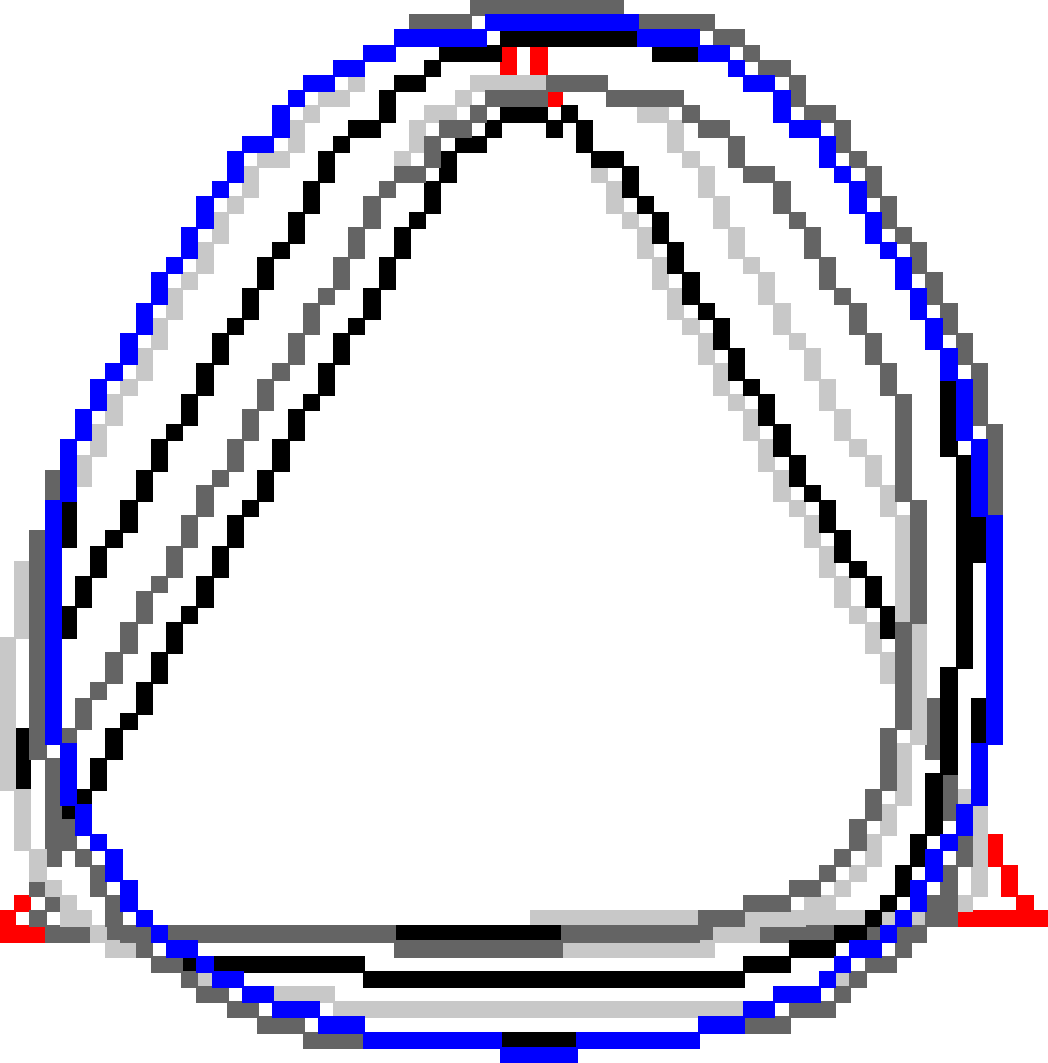
\includegraphics[scale=0.185]{figures/chapter5/exhaustive-selection/mdca-lp0.01/triangle/summary.pdf}\\[2em]
	
	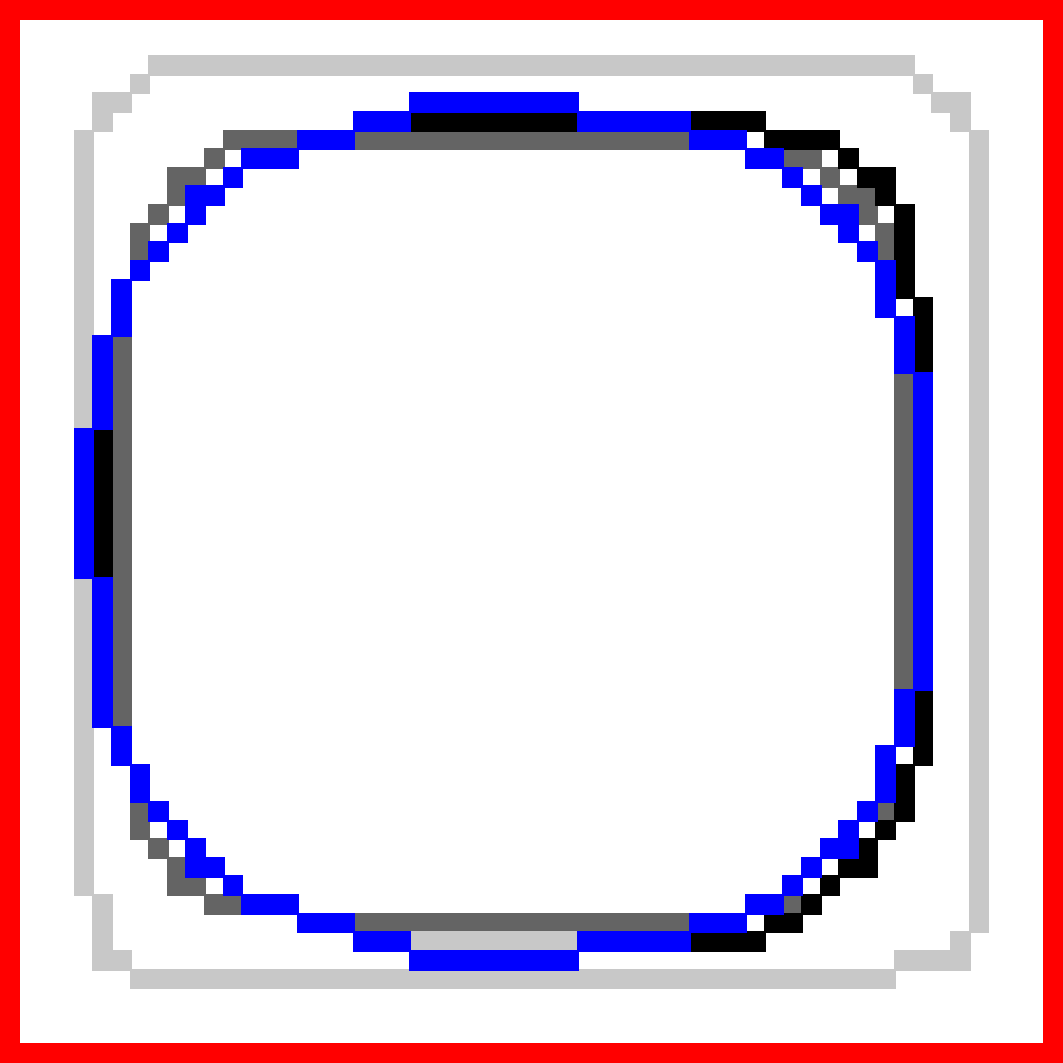
\includegraphics[scale=0.17]{figures/chapter5/exhaustive-selection/mdca-lp0.01/square/summary.pdf}\\[2em]
	
	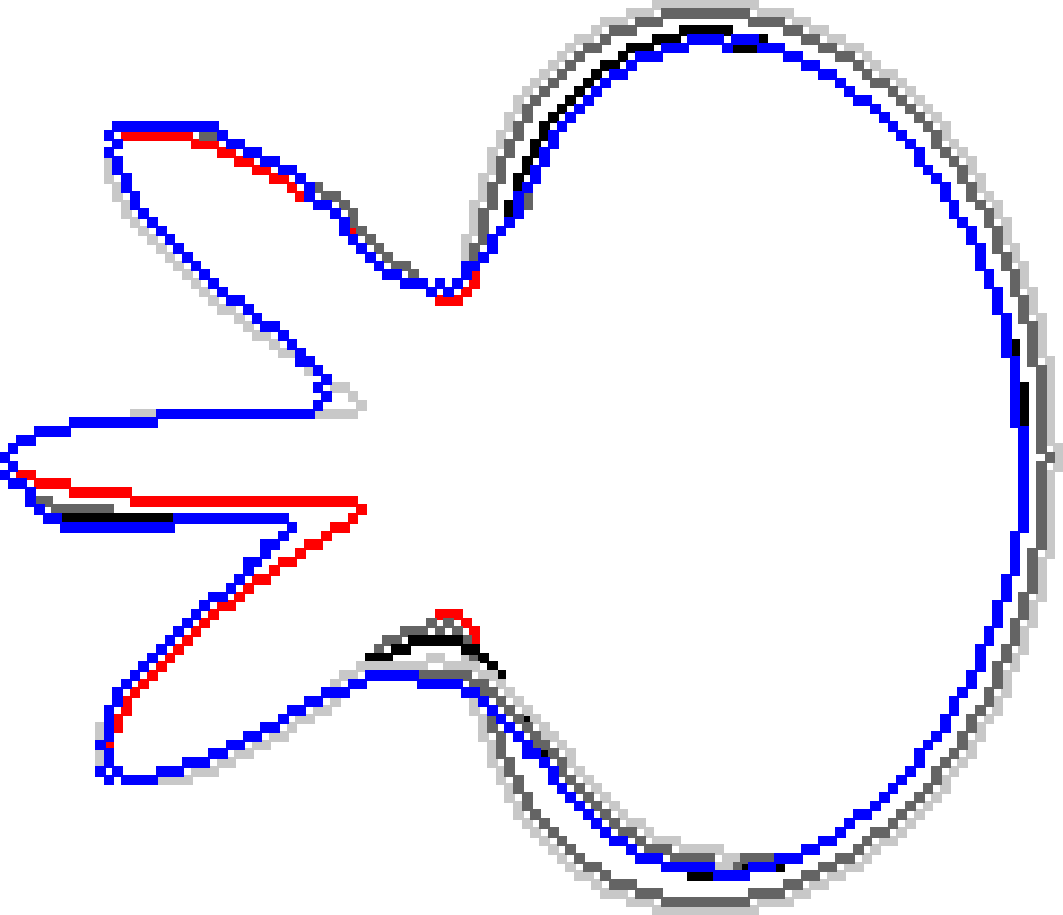
\includegraphics[scale=0.25]{figures/chapter5/exhaustive-selection/mdca-lp0.01/flower/summary.pdf}\\[2em]

	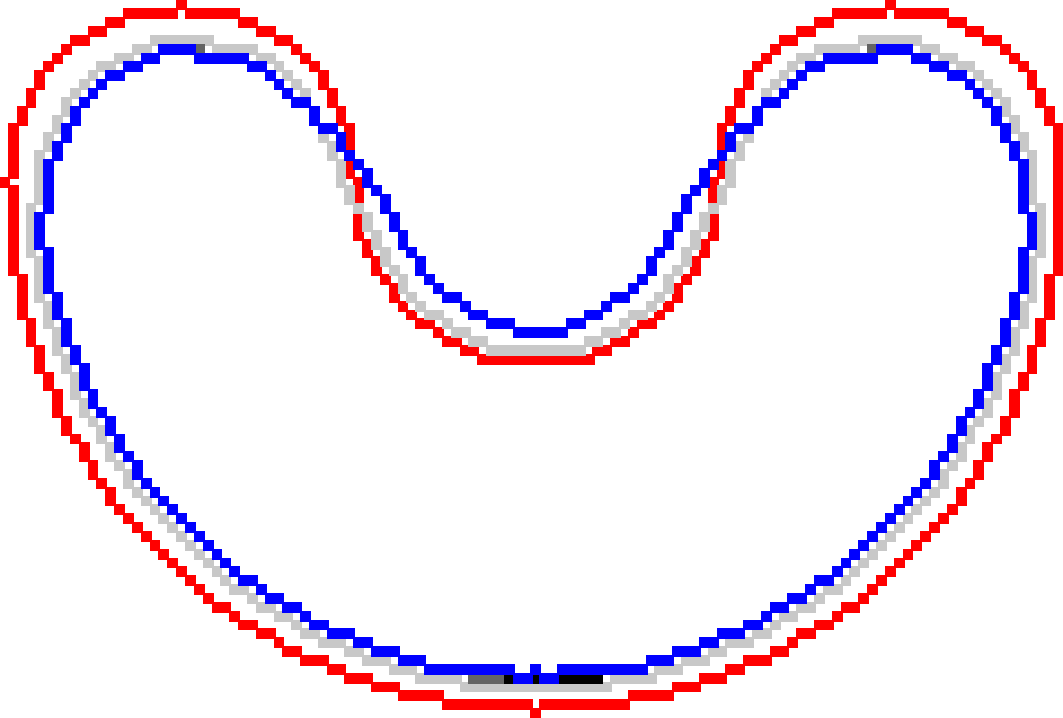
\includegraphics[scale=0.25]{figures/chapter5/exhaustive-selection/mdca-lp0.01/bean/summary.pdf}
\end{minipage}%	
		\caption{Local combinatorial optimization process results for several shapes with $\alpha=0.01,\beta=1$. In the left column we have evolutions using II-$5$ and in the right MDCA. Shapes are displayed at every $5$ iterations.}	
		\label{fig:local-comb-square-results}
\end{figure}


\begin{figure}[h!]
\center
\captionsetup{type=table}
\begin{tabular}{|l|c|c|c|c|c|c|}
\hline
& \multicolumn{2}{c|}{$h=1.0$} & \multicolumn{2}{c|}{$h=0.5$} & \multicolumn{2}{c|}{$h=0.25$}\\
\hline
& Pixels & Time & Pixels & Time & Pixels & Time\\
\hline
Triangle & 131 & 1s (0.1s/it)  & 521 & 72s (2.7s/it) & 2080 & 1300s (18s/it)\\
Square & 225 & 1s (0.1s/it) & 841 & 16s (0.9s/it) & 3249 & 656s (9.9s/it)\\
Flower & 469 & 14s (1s/it) & 1867 & 218s (6.4s/it) & 7481 & 3246s (42s/it)\\
Bean  & 1574 & 74s (1.9s/it) & 6278 & 995s (12.9s/it) & 25130 & 28580s (95.5s/it)\\
\hline
\end{tabular}
\caption{Running time and input size for different grid steps.}
\label{tab:summary-local-comb-rtime} 
\end{figure}






The algorithm is suitable for any type of digital estimators. To estimate length we use MDSS and to estimate curvature we execute experiments with the MDCA and II-$5$ estimators. We observe that II-$5$ evolves the triangle, the square and the flower to the optimal disk of radius $10$. On the other hand, MDCA evolution get stucked in local optima. In fact, the MDCA estimator, although with higher convergence speed, is more sensitive to noise than II, as illustrated in figure \ref{fig:mdca-sensitivity}. For the bean shape, both estimators stop in a local optima. In figure \ref{fig:local-comb-plots}, we can observe how the elastica value evolves for each shape and each curvature estimator.








\begin{figure}[h!]
\begin{minipage}[b]{0.6\textwidth}
\center
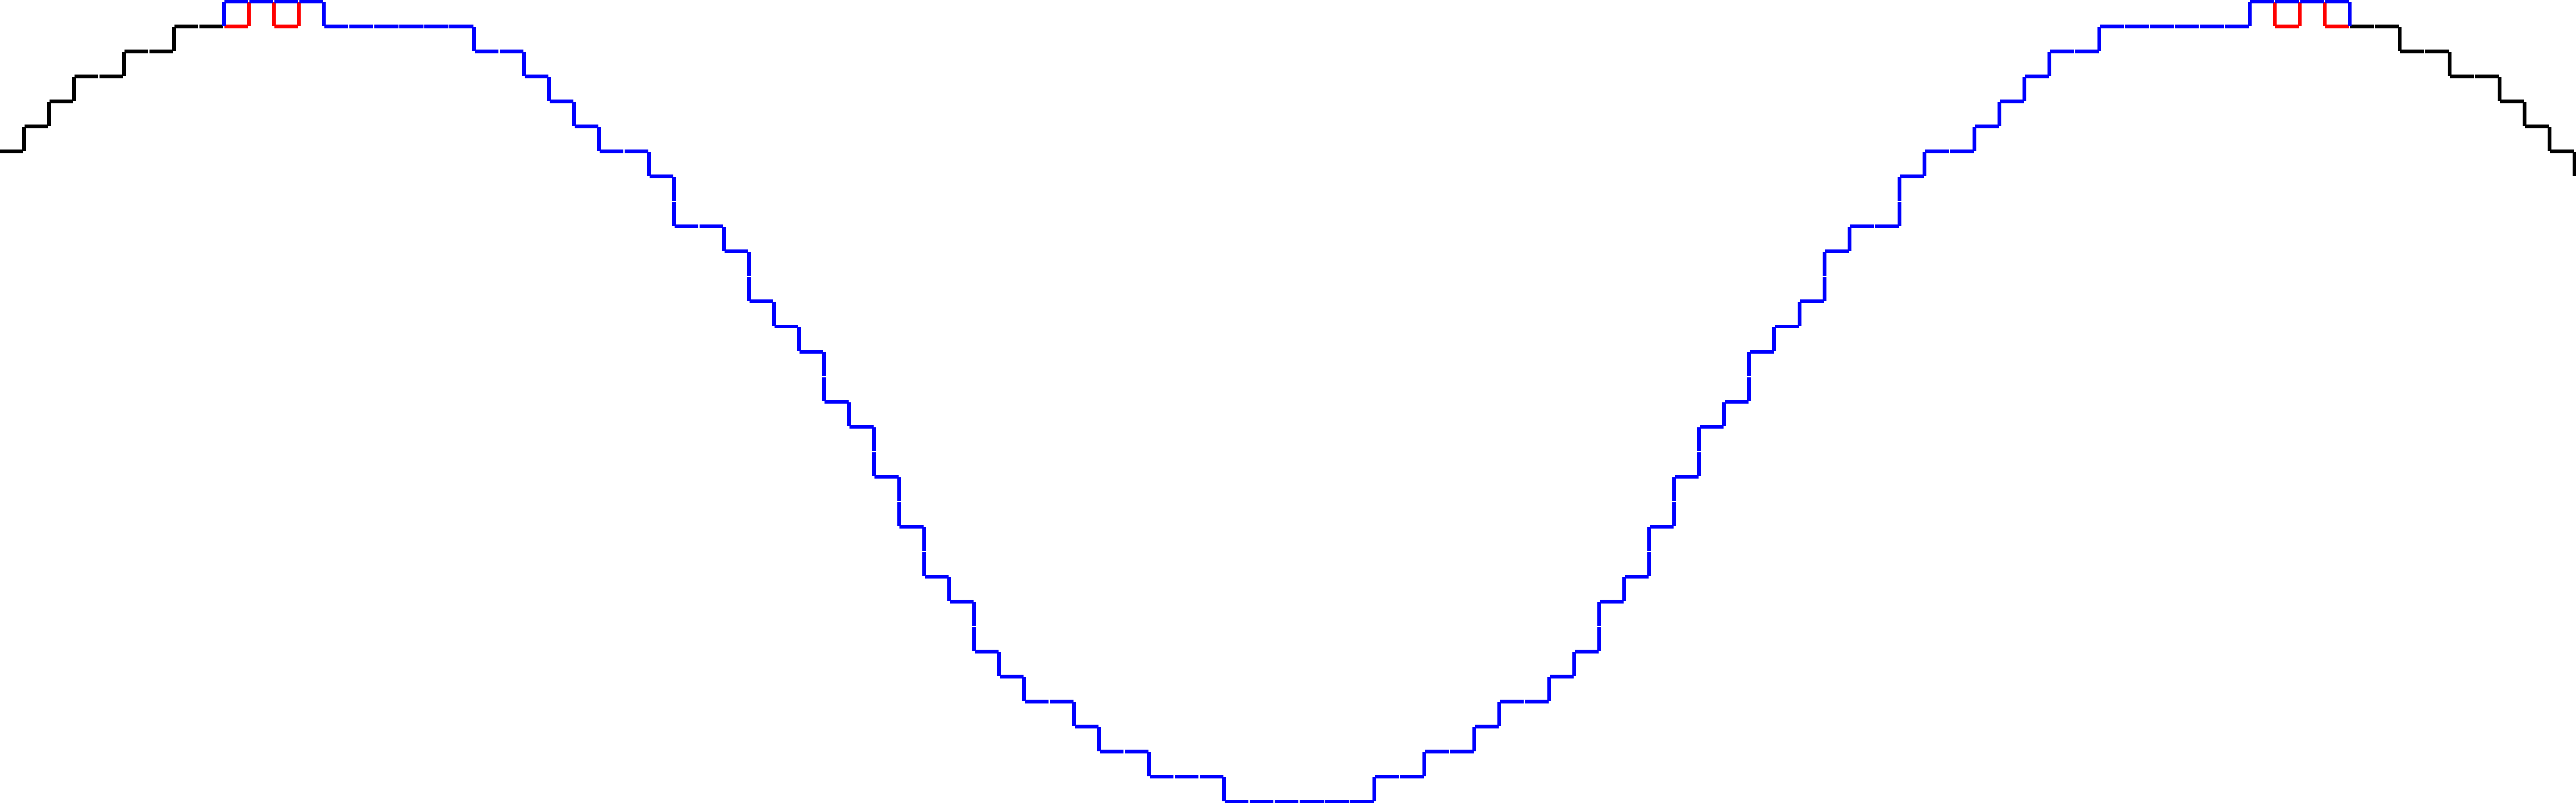
\includegraphics[scale=0.15]{figures/chapter5/mdca-sensitivity/closer-picture.pdf}
\end{minipage}%
\begin{minipage}[b]{0.4\textwidth}
\center
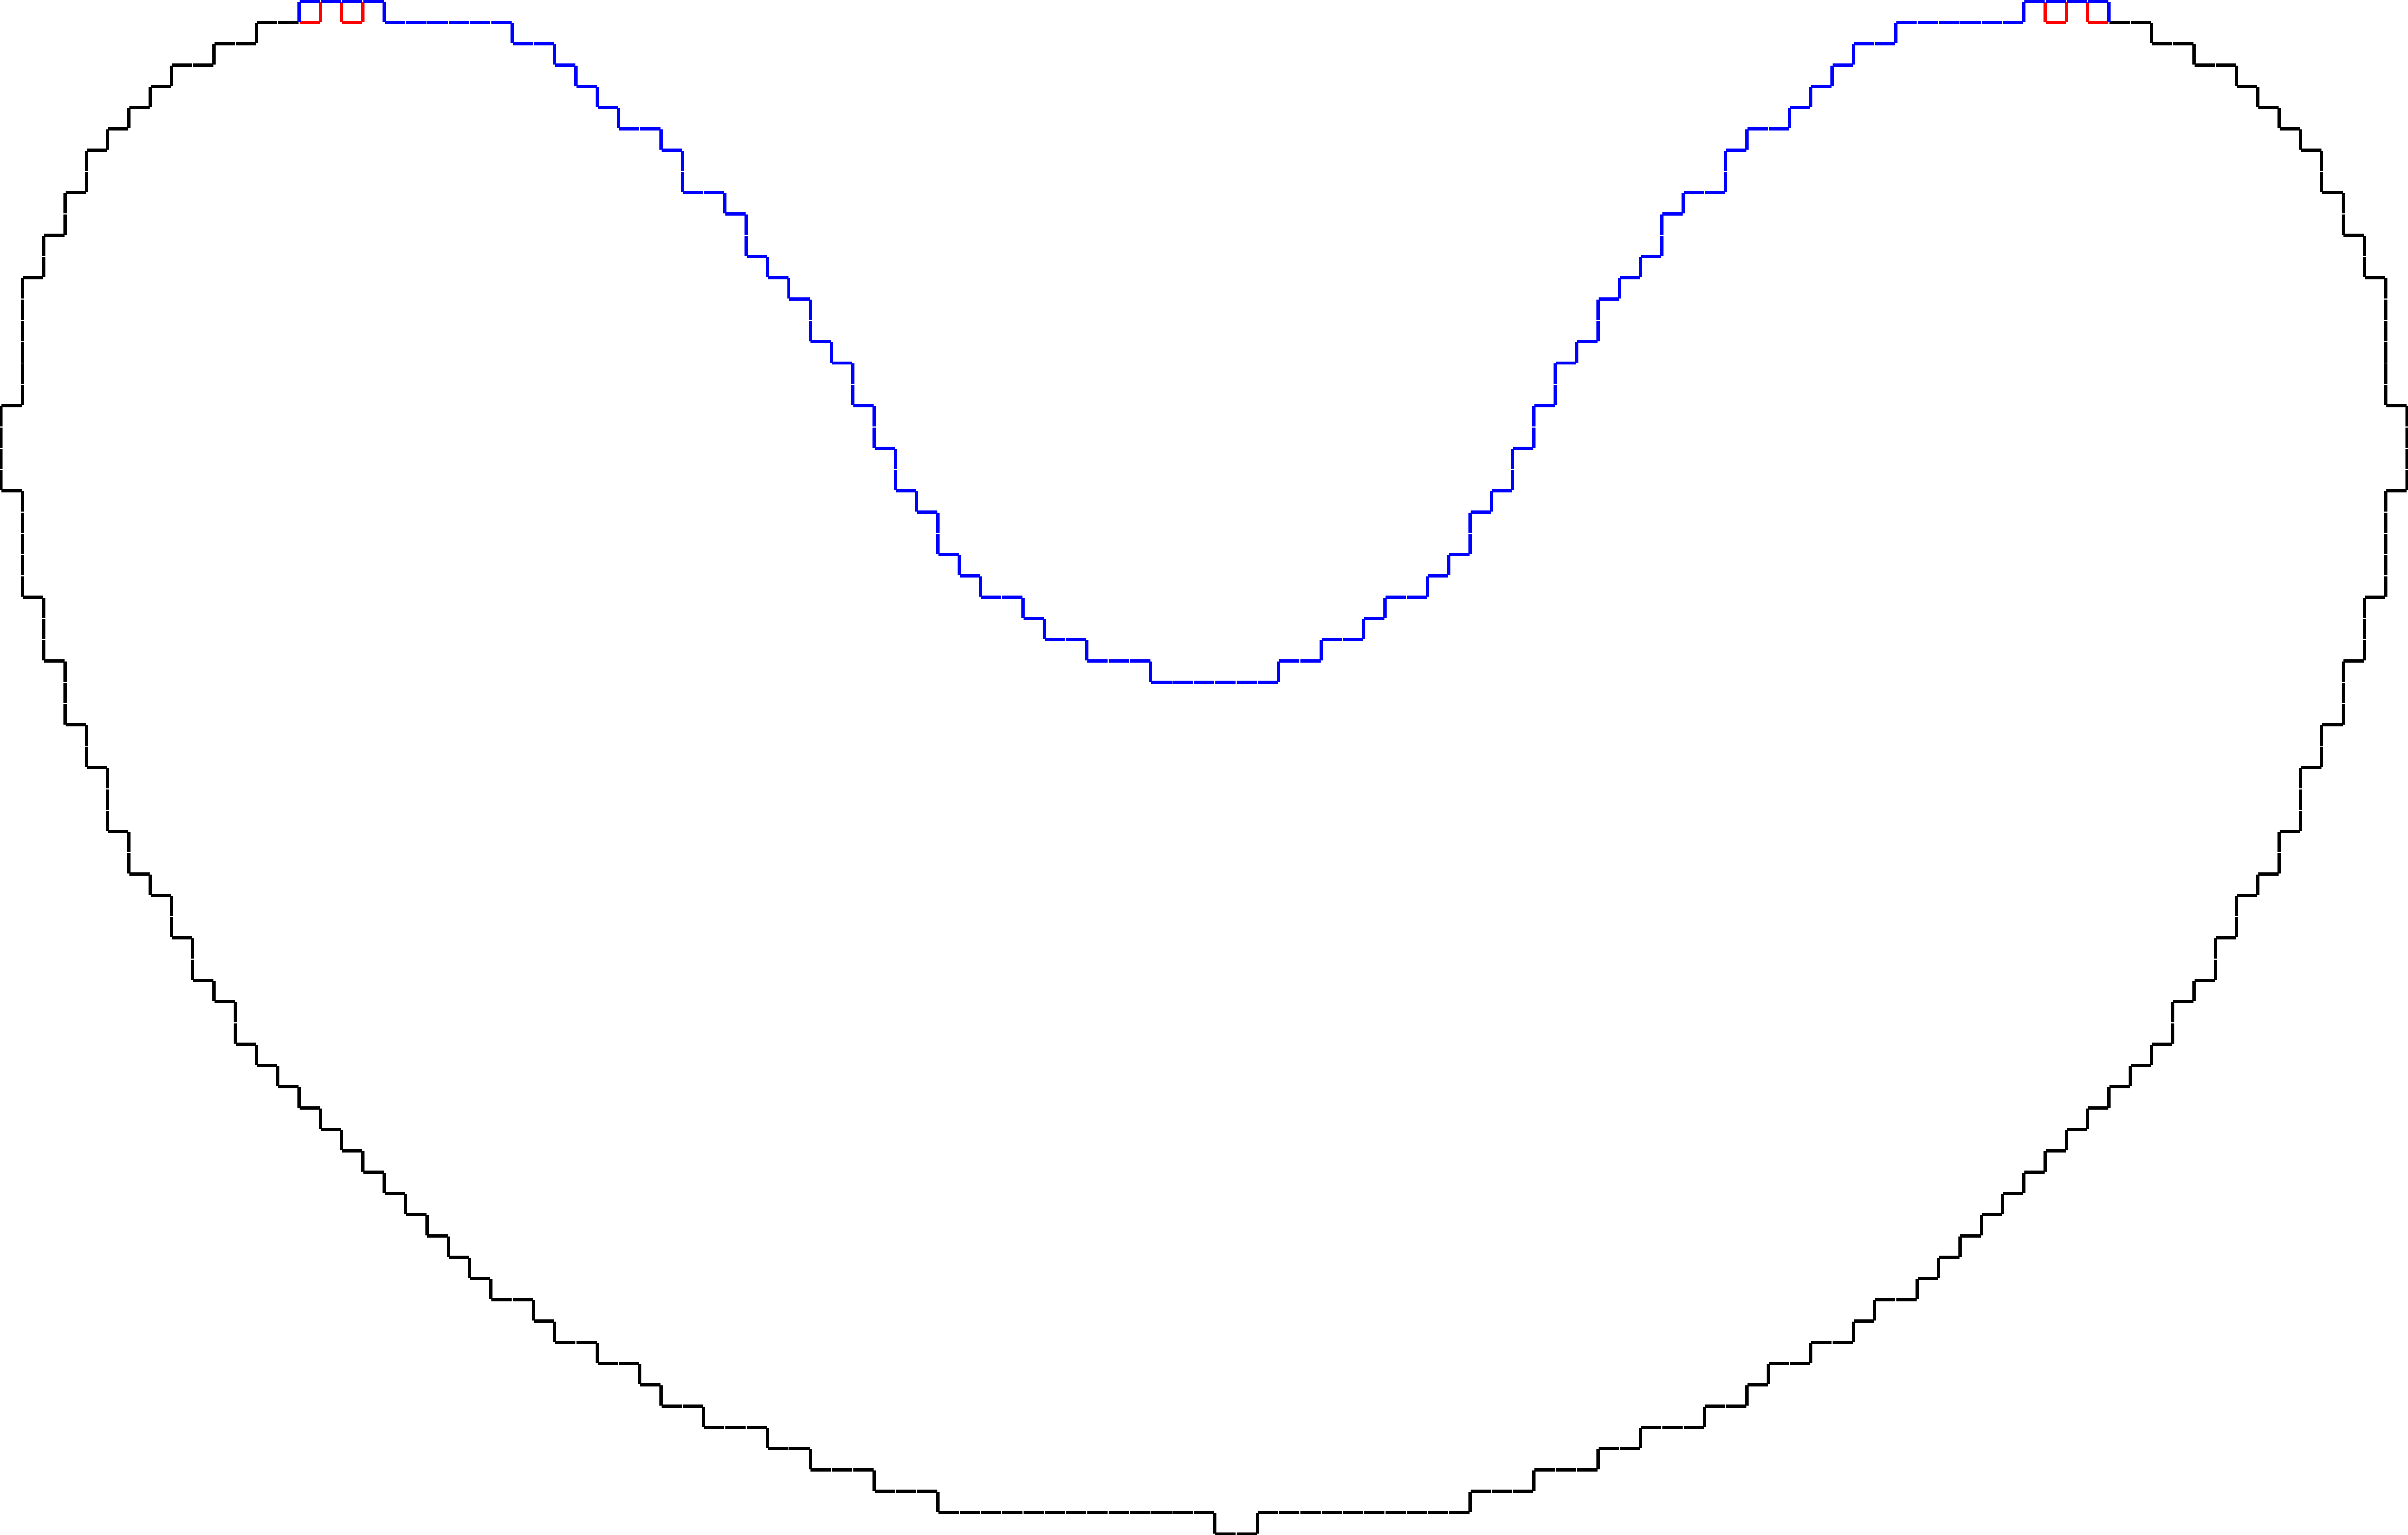
\includegraphics[scale=0.025]{figures/chapter5/mdca-sensitivity/big-picture.pdf}\\\vspace{2em}
\captionsetup{type=table}
\begin{tabular}{r|c|c}
& II-$5$ & MDCA \\
\hline
Red  & 5.54 & 3.93\\
Blue & 5.55 & 3.84\\
\hline
$| \Delta E / \Delta S |$ & 70 & 1400
\end{tabular}
\end{minipage}
\caption{A slight variation in the shape boundary (in this example, a $0.07\%$ change or $4$ pixels over $5310$) inflicts a considerably higher change in the energy value when using MDCA than when using II. }
\label{fig:mdca-sensitivity}
\end{figure}





The running time of algorithm \ref{alg:local-search} is summarized in table \ref{tab:summary-local-comb-rtime}. All the experiments in this paper were executed on a $32$-core $2.4Ghz$ CPU. Although its use in practical applications is
limited, we demonstrate that digital estimators are effective in their measurements and the flows evolve as expected, reaching the global optima for some shapes. We
observe that it is a complete digital approach, and we do not suffer from discretization and rounding problems, a common
issue in continuous models.  Furthermore we have checked that this approach works indifferently with Integral Invariant
curvature estimator and Maximal Digital Circular Arc curvature estimator. So the convergence of the digital curvature
estimator seems to be the cornerstone to get a digital curve behaving like a continuous Elastica.  

We can also impose some restrictions in the evolution process. For example, we can force some pixels to be part of the final shape, or that the endpoints of the curve must have a given orientation. Figure \ref{fig:fixed-pixels-evolution} summarizes the results.

\begin{figure}[h!]
\center
\subfloat[\label{fig:fixed-a}]{
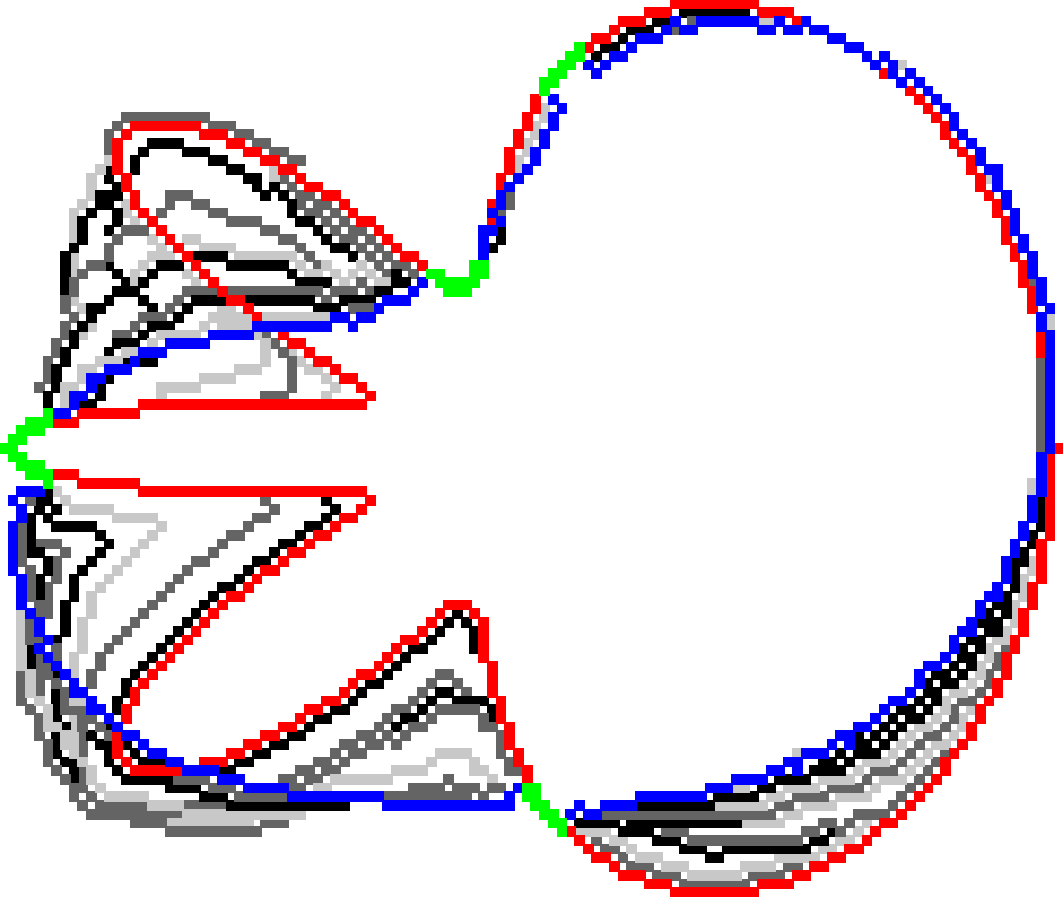
\includegraphics[scale=0.25]{figures/chapter5/fixed-pixels/flower-1/summary.pdf}
}\hspace{1em}%
\subfloat[\label{fig:fixed-b}]{
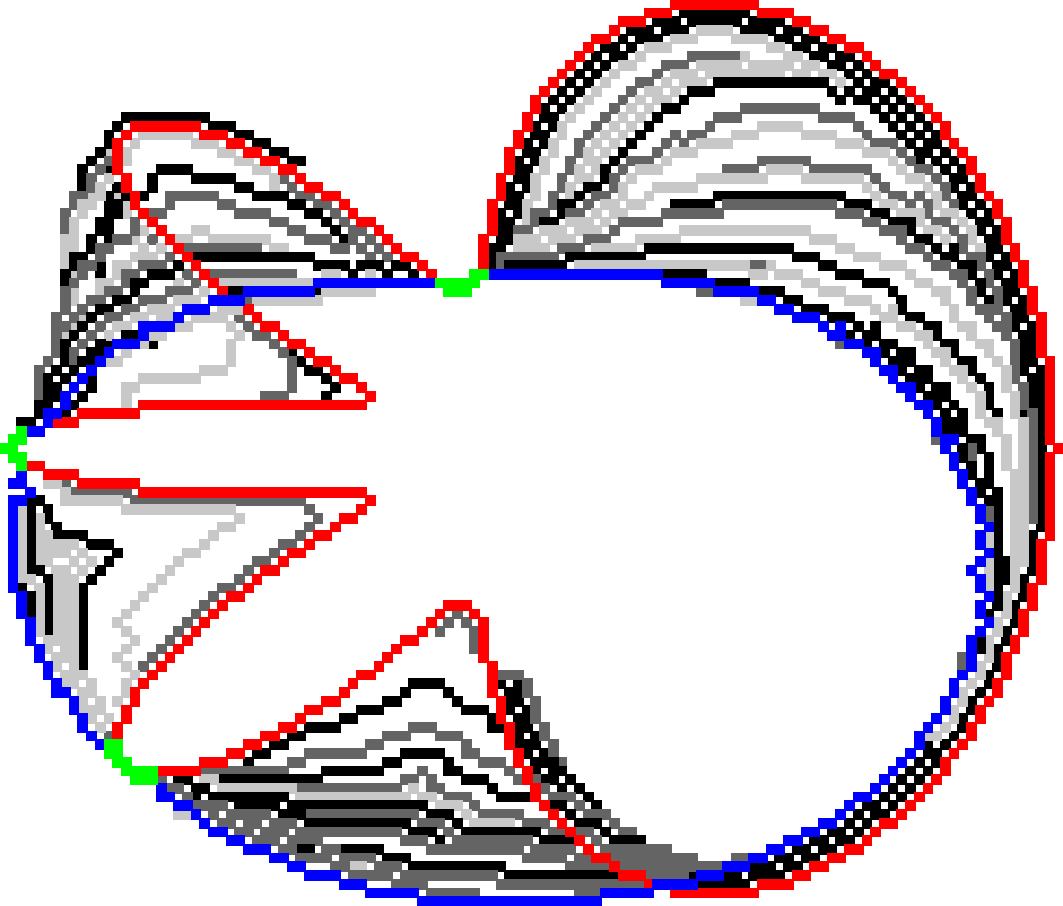
\includegraphics[scale=0.25]{figures/chapter5/fixed-pixels/flower-2/summary.pdf}
}\hspace{1em}%
\subfloat[\label{fig:fixed-c}]{
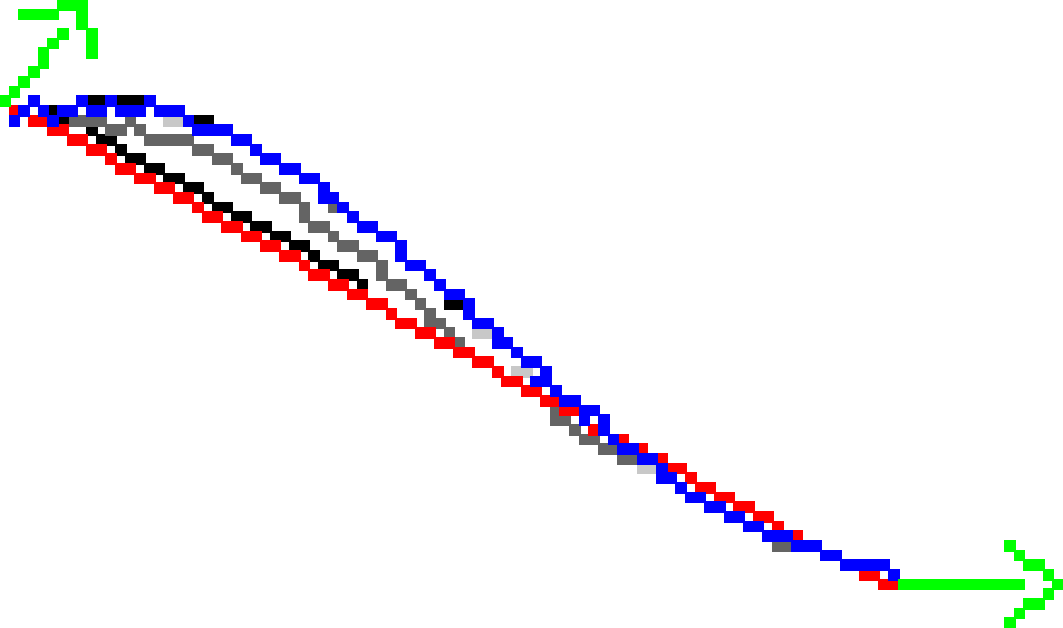
\includegraphics[scale=0.25]{figures/chapter5/fixed-orientation/pair-1/summary.pdf}
}\hspace{1em}%
\subfloat[\label{fig:fixed-d}]{
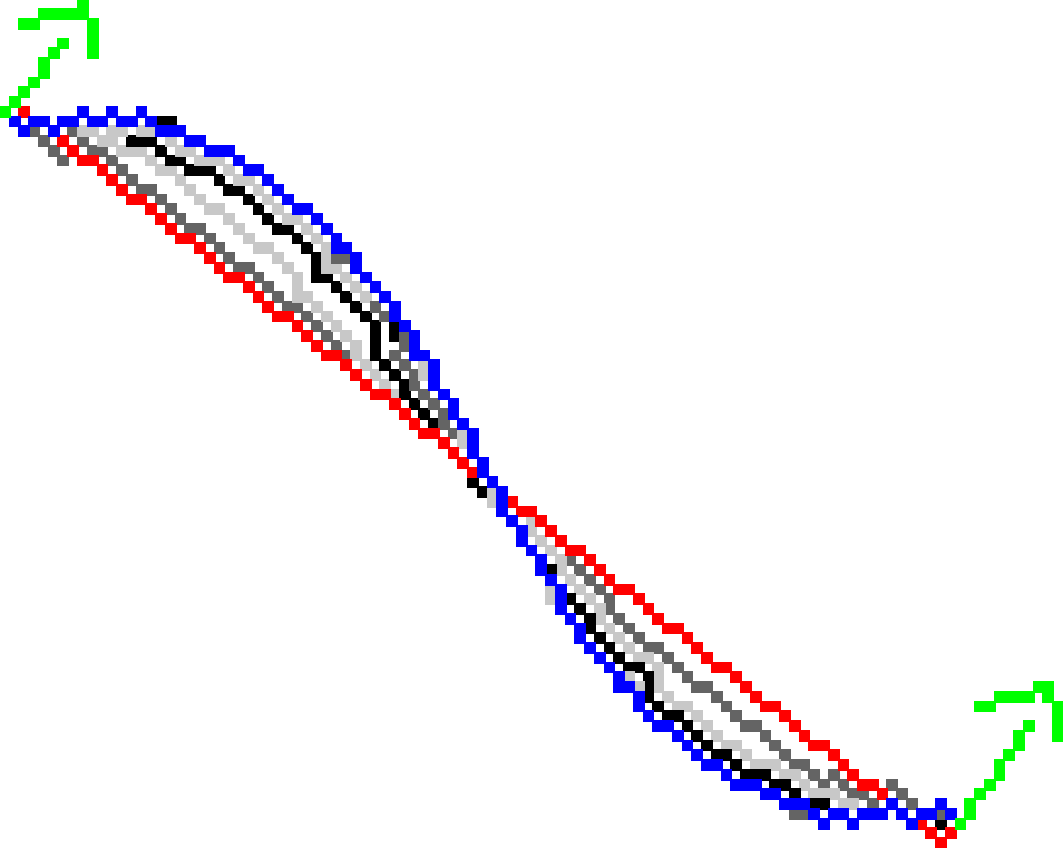
\includegraphics[scale=0.25]{figures/chapter5/fixed-orientation/pair-2/summary.pdf}
}\hspace{1em}%
\subfloat[\label{fig:fixed-e}]{
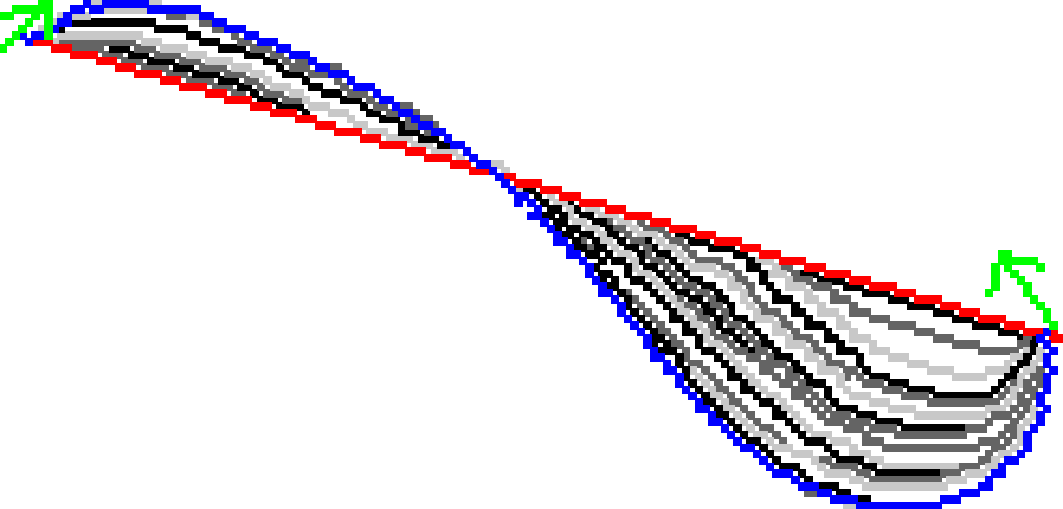
\includegraphics[scale=0.25]{figures/chapter5/fixed-orientation/pair-3/summary.pdf}
}\hspace{1em}%

\caption{Green segments denote pixels to be enforced in the final shape for figures (a) and (b); or fixed orientations in the endpoints of an open curve as in figures (c)-(e). }
\label{fig:fixed-pixels-evolution}
\end{figure}

We also evaluate the process for a simplified version of the elastica in which the local length estimator is ommited

	\begin{align}
	\hat{E}_S( D_h(X) ) = \sum_{\dot{\vec{e}} \in \partial D_h(X)}{ \alpha + \beta \hat{\kappa}_{r}^2(D_h(X),\dot{\vec{e}},h) }.
	\label{eq:simplified-digital-elastica}
	\end{align}
	

\begin{figure}[h!]
\center
\subfloat[\label{fig:fixed-a}]{
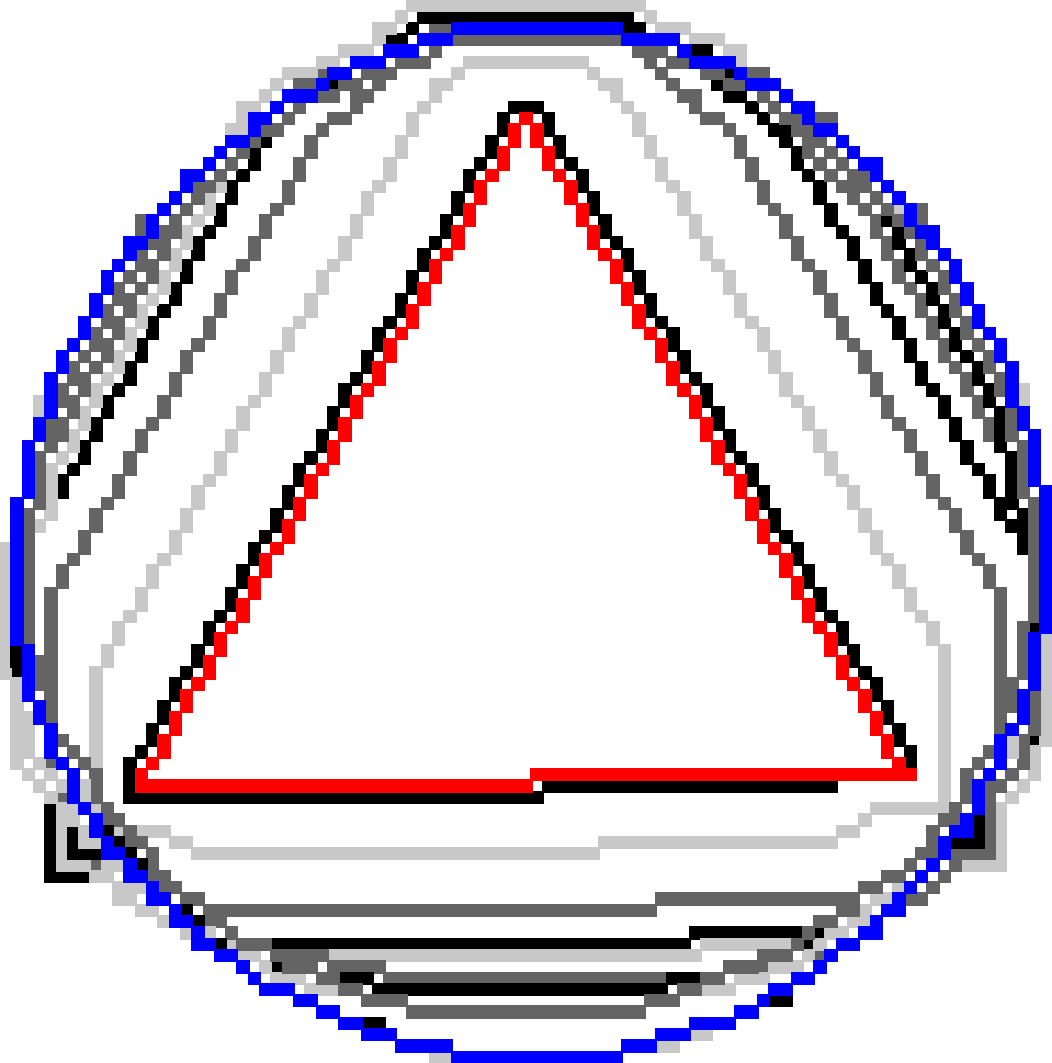
\includegraphics[scale=0.185]{figures/chapter5/sqc/flow/triangle/summary.pdf}
}\hspace{1em}%
\subfloat[\label{fig:fixed-b}]{
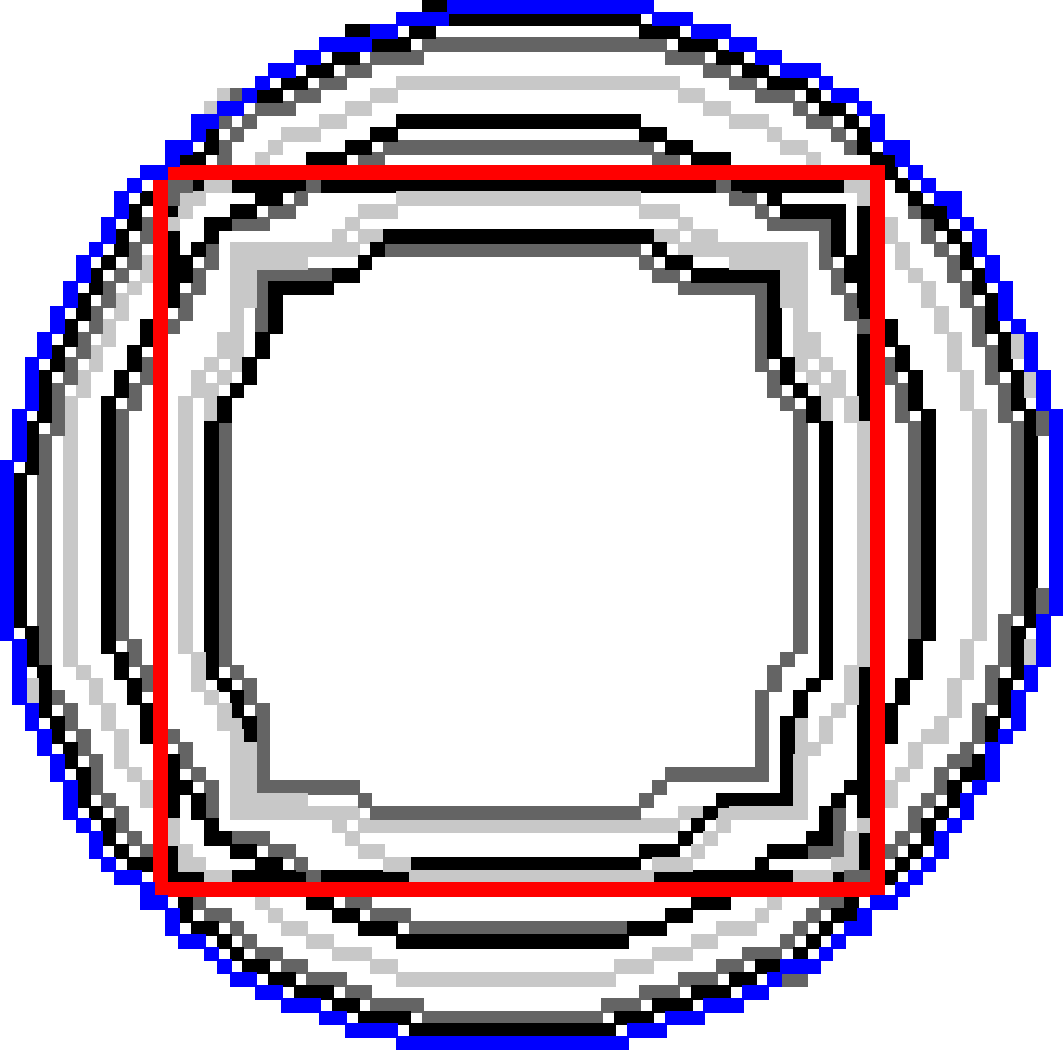
\includegraphics[scale=0.17]{figures/chapter5/sqc/flow/square/summary.pdf}
}\hspace{1em}%
\subfloat[\label{fig:fixed-d}]{
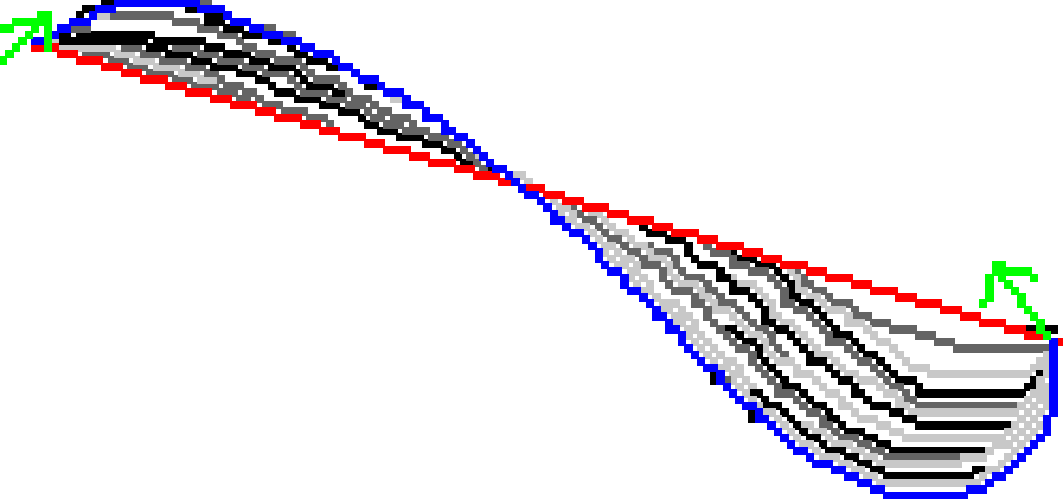
\includegraphics[scale=0.25]{figures/chapter5/sqc/fixed-orientation/pair-3/summary.pdf}
}
\caption{Simple elastica experiments}
\label{fig:simple-elastica-experiments}
\end{figure}

We obtain similar results for the previous experiments (see figure \ref{fig:simple-elastica-experiments}), except when handling the flower shape. Flow evolution for smoother versions of the flower doesn't change this scenario, which suggests that the simplified flow is not suited for initial shapes with regions of negative curvature.

In fact, the defined neghborhood is likely to not be appropriate for the simple elastica. Let $\{S_i\}$ be the sequence of shapes generated by algorithm \ref{alg:local-search} using digital elastica \eqref{eq:digital-elastica} and $\{Q_i\}$ the sequence of shapes generated by the same algorithm but using the simplified version of elastica \eqref{eq:simplified-digital-elastica}. Both sequences starts from the flower shape, i.e. $S_0=Q_0=flower(0.25)$. In figure \ref{} we compute the simple elastica energy for $\{S_i\}$ and $\{Q_i\}$ and we notice that the lowest values are achieved for $\{S_i\}$, except at the first iterations. That suggests that by using a larger neighborhood, the simplified elastica can be employed as a reasonable approximation of \eqref{eq:digital-elastica}. In particular, energy \eqref{eq:simplified-digital-elastica} is suitable for a global optimization model.


\begin{figure}[h!]
\center
\label{fig:sqc-energy-experiments}	
\subfloat[\label{fig:fixed-c}]{
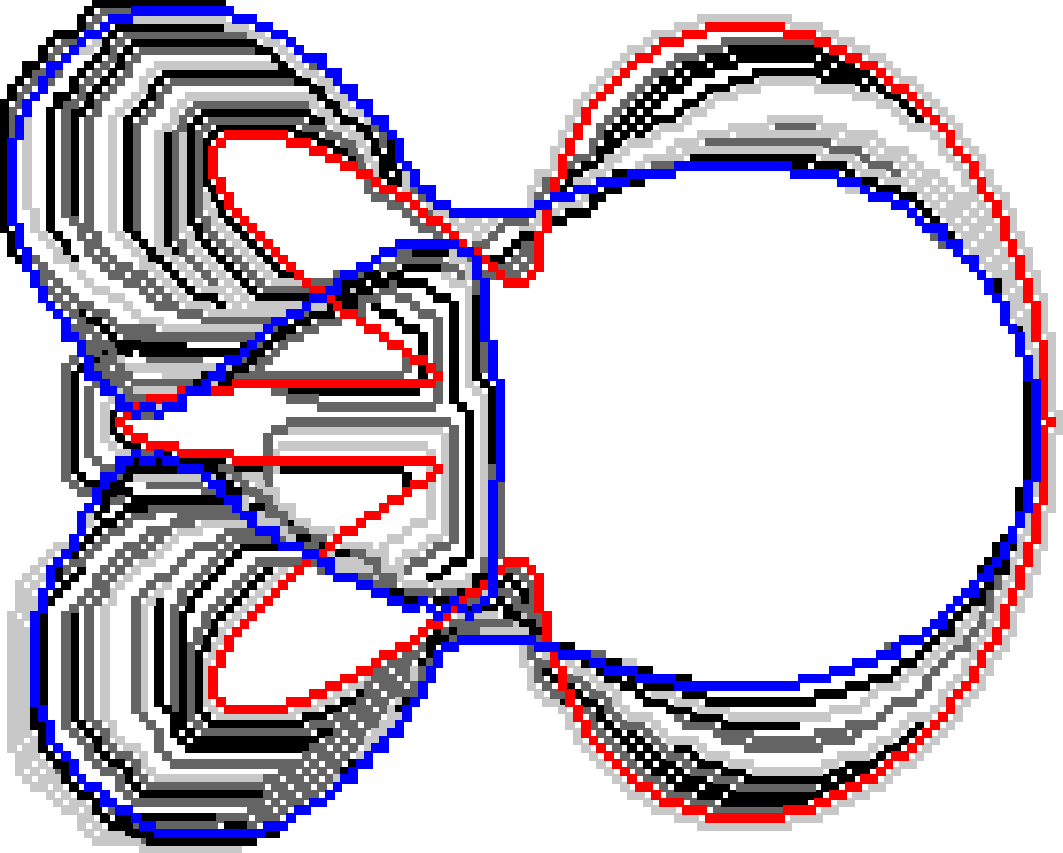
\includegraphics[scale=0.25]{figures/chapter5/sqc/flow/flower/summary.pdf}
}\hspace{1em}%
\subfloat[\label{fig:fixed-c}]{
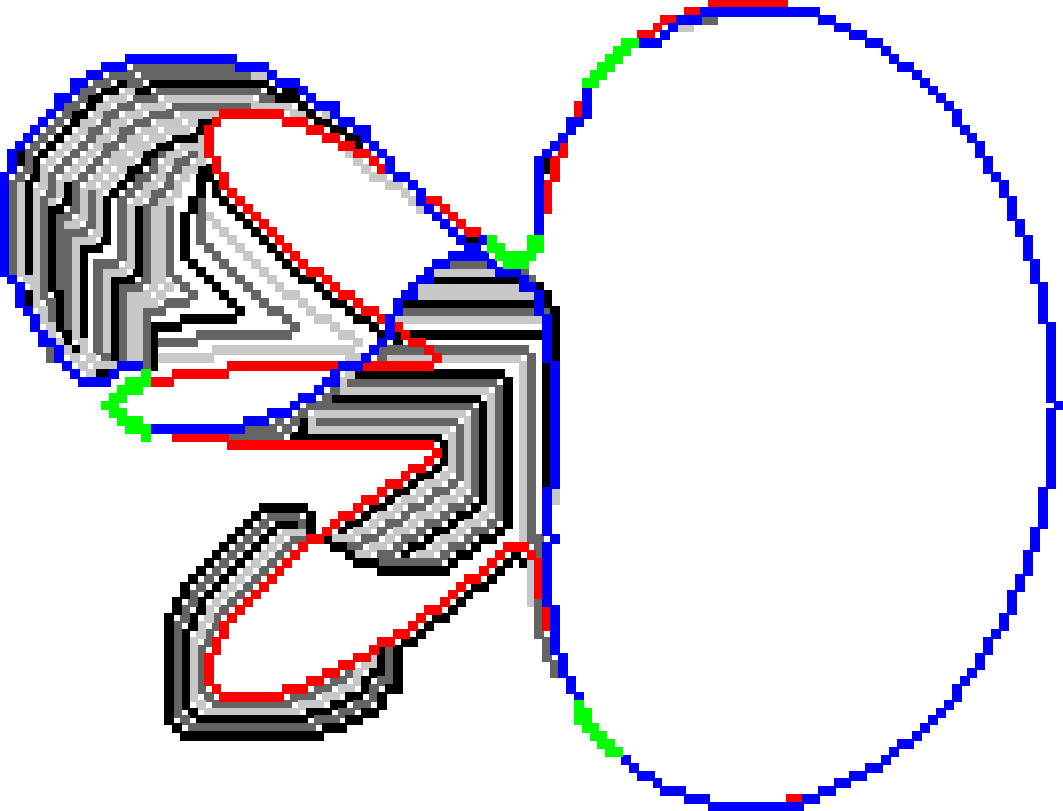
\includegraphics[scale=0.25]{figures/chapter5/sqc/fixed-points/flower-1/summary.pdf}
}\hspace{1em}%
\subfloat[\label{fig:fixed-c}]{
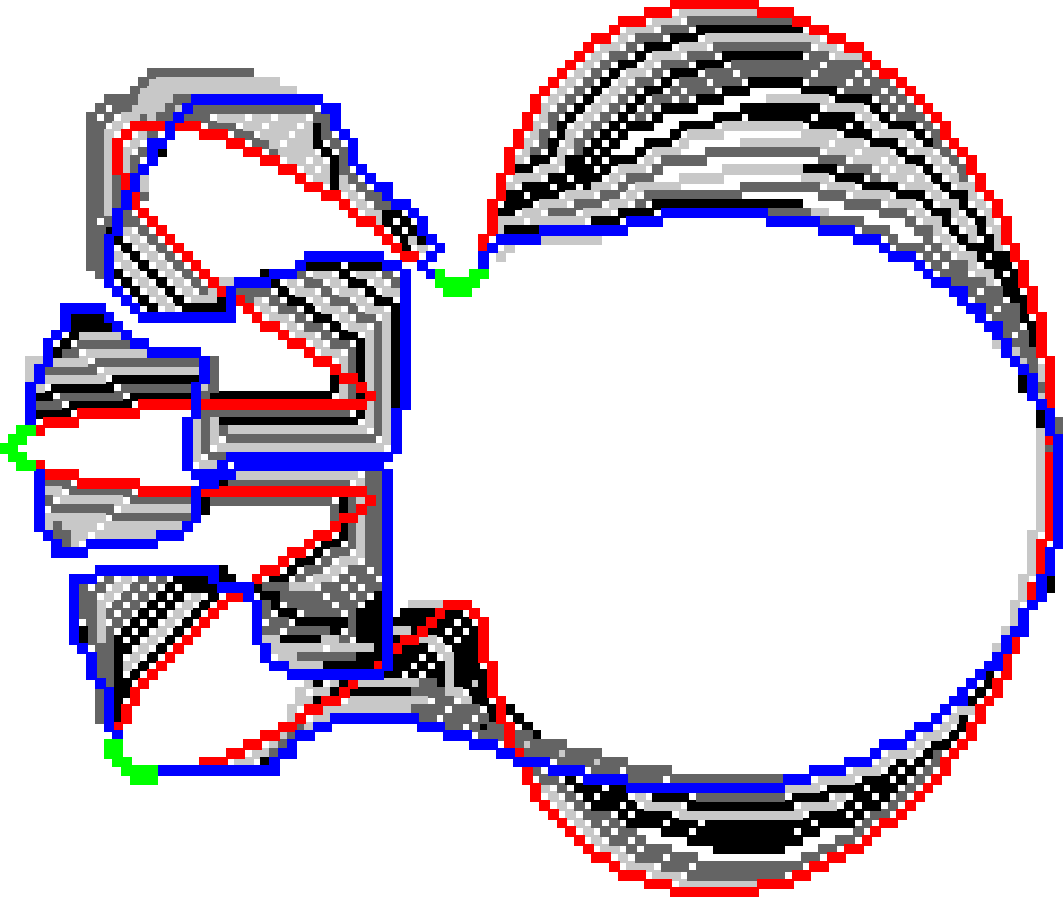
\includegraphics[scale=0.25]{figures/chapter5/sqc/fixed-points/flower-2/summary.pdf}
}\\
\subfloat[\label{fig:fixed-c}]{
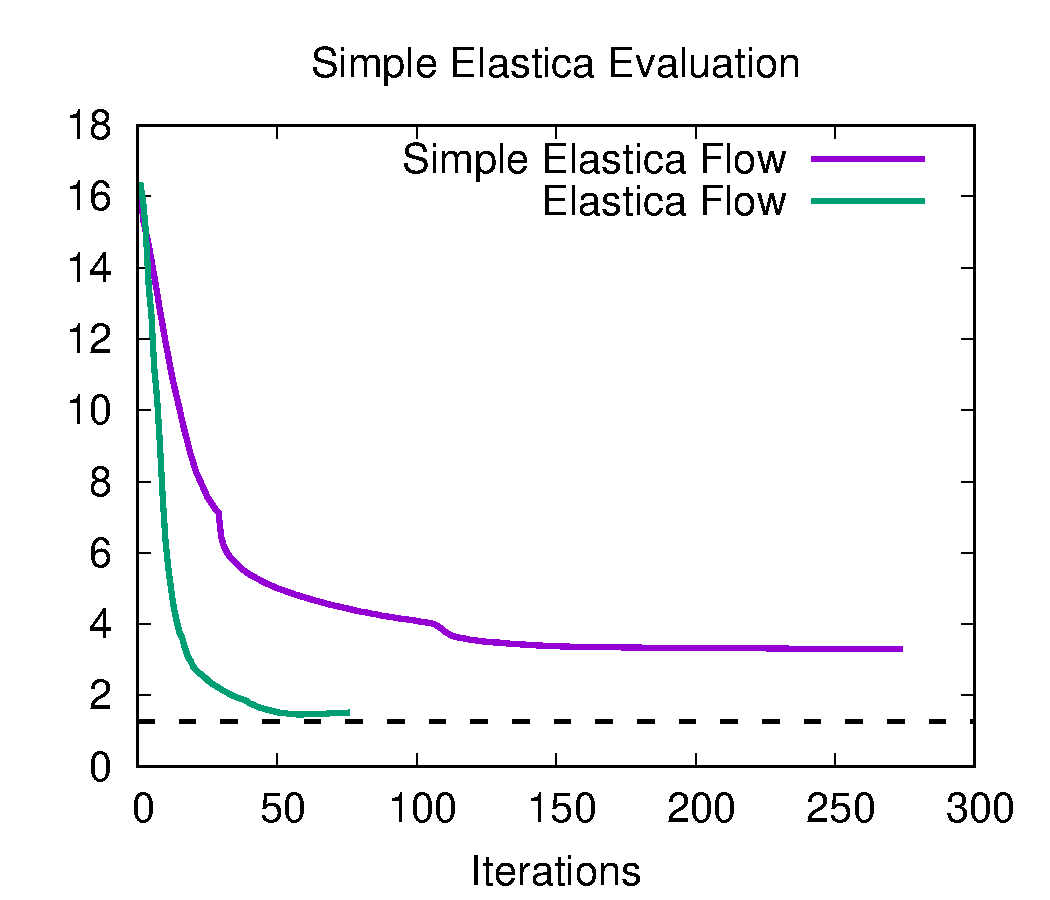
\includegraphics[scale=0.28]{figures/chapter5/sqc/plots/flow-flower.pdf}
}\hspace{0.25em}%
\subfloat[\label{fig:fixed-c}]{
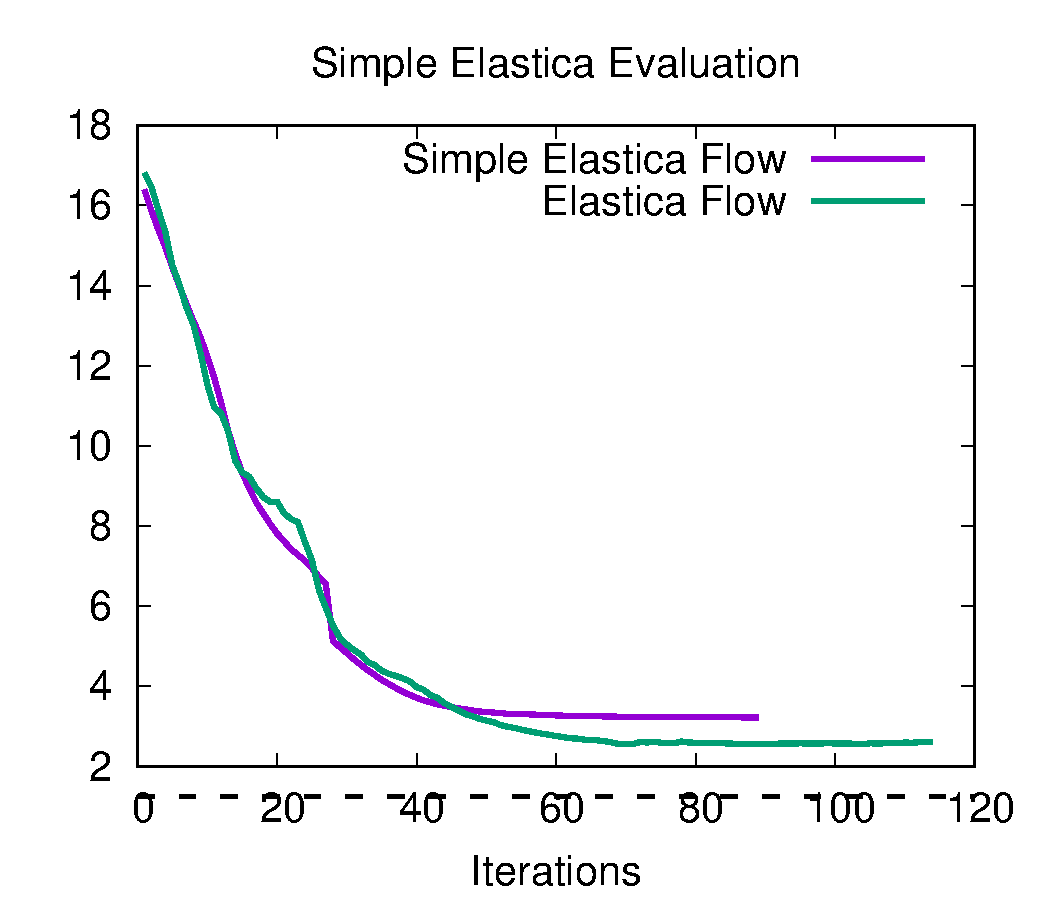
\includegraphics[scale=0.28]{figures/chapter5/sqc/plots/fixed-flower-1.pdf}
}\hspace{0.25em}%
\subfloat[\label{fig:fixed-c}]{
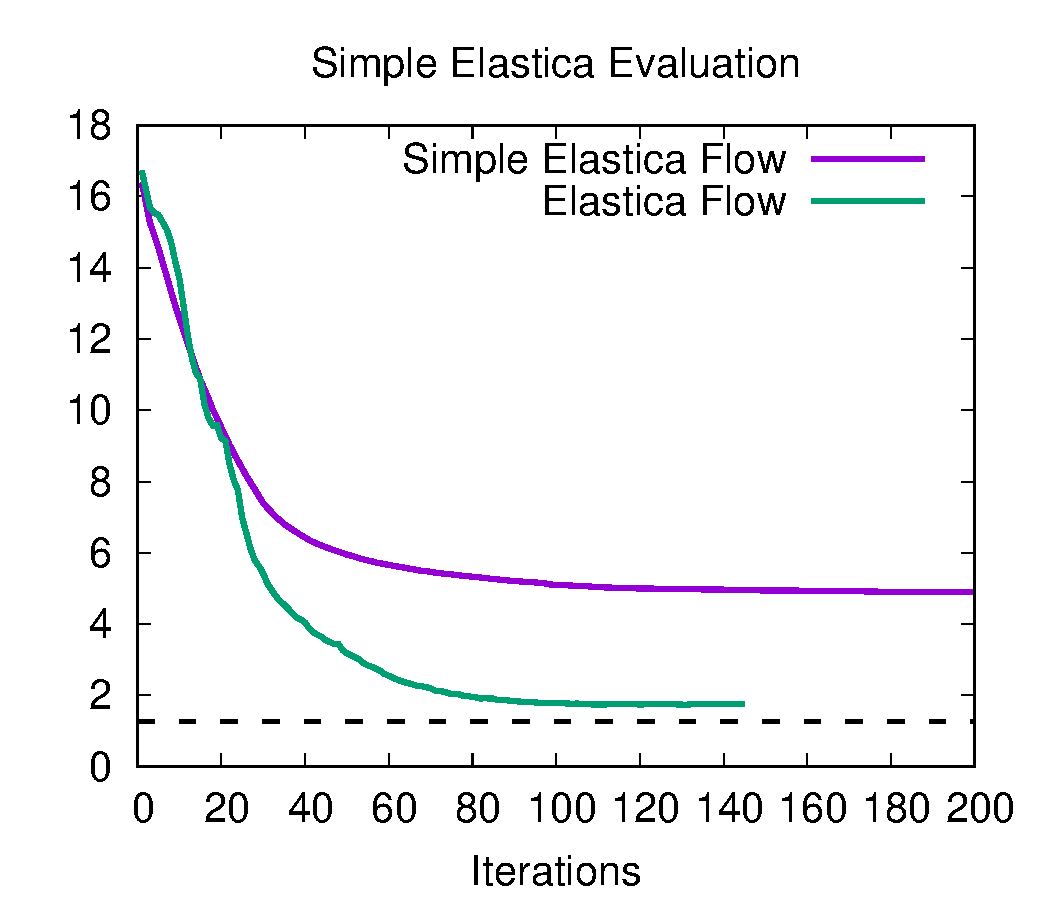
\includegraphics[scale=0.28]{figures/chapter5/sqc/plots/fixed-flower-2.pdf}
}
\end{figure}

\section{Global Optimization Model}

Differently from the previous section, the model described here is designed for the integral invariant estimator only. Let $D \in \frac{1}{2}\mathbb{Z}^2$ be the digitization of some shape $S \in \mathbb{R}^2$ using grid step $h$ in half-integer coordinates space. We assume that $D$ has $m$ pixels (located at integer coordinates) and $n$ linels (one and only one of its coordinates is $\frac{1}{2}$). Optimization variables are represented as vectors $x \in \mathbb{B}^{m},\, y \in \mathbb{B}^{n}$ and its $i$th coefficients denoted  $x_i,y_i$.  Further, let $A \in \mathbb{B}^{m\times n}$ the matrix defined as

\[
	A_{i,j} = \left\{ \begin{array}{ll}
		1,\; x_j \in B_{r}(y_i)\\
		0,\; \text{otherwise}.
	\end{array}\right.
\]

In other words, the column vector $A_i$ of $A$ represents the pixels that are in the interior of  the disk $B_{r}(y_i)$ of radius $r$ centered at $y_i$. 


\begin{align}
	\hat{E}(x,y) =& \sum_{y_i \in y}{ y_i \left(\; \alpha + \beta \hat{\kappa}_{r}^2(D,y_i) \; \right)}\\\nonumber
			   =& \sum_{y_i \in y}{ y_i \left(\; \alpha  + \beta \big( \frac{3}{r^3}(\frac{\pi}{r^2} - |B_r(y_i)|)\big)^2\right)}\\\nonumber
			   =& \sum_{y_i \in y}{ y_i \left(\; \alpha + \frac{9}{r^6}\beta \big(c^2 - 2cA_i^T\vec{x} + \vec{x}^TA_iA_i^T\vec{x}\big)\right)},			   
	\end{align}
	
where $c =  \pi r^2/2$. We remark that linels and pixels in the solution must be topologicaly consistent, .i.e., linels must form connected closed curves and the pixels must lie in the interior of those curves. This restriction is encoded in a set of constraints $C(x,y)$ detailed later. So far we have

\begin{align*}
	\min_{x \in \mathbb{B}^{|X|}, y \in \mathbb{B}^{|Y|}}{\hat{E}(x,y)}, \quad \text{subject to } C(x,y). \quad (P0)
\end{align*}

The continuous counterpart of $P0$ has a very intuitive interpretation. We know that the shape that minimizes the integration of squared curvature is the ball of infinite radius. On the other hand, we know that the flow derived from perimeter minimization is the curvature flow, which invariably reaches a disk before converging to a single point. Therefore, we can expect that the global optima for $P0$ will be a disk. Hence, it is sufficient to analyze what it happens by restricting $P0$ to disks

\begin{align*}
	\frac{d}{dr}\big( \alpha 2\pi r + \beta \pi/r \big) &= 0\\
	r &= \alpha^{-1/2}.
\end{align*}  

We conclude that the solution for problem $P0$ is the ball of radius $\alpha^{-1/2}$. In real applications involving the minimization of elastica, we have an additional set of constraints $R$ that plays the role of regularization. For example, we may force some of the pixels in the original shape to be part of the solution; for imaging problems, we may add a data attachment term, and so on. Finally, we can write the general optimization problem as

\begin{align*}
	\min_{x \in \mathbb{B}^{|X|}, y \in \mathbb{B}^{|Y|}}{\hat{E}(x,y)}, \quad \text{subject to } C(x,y), R(x) \quad (P1)
\end{align*}

	Formulation $P1$ is a constrained binary non-convex third order problem and likely difficult to be solved optimally. Nonetheless, we can use standard optimization techniques to acquire some intuition on the model. 	
	
\subsection{Topological constraints}



The aim of the topological constraints is to enforce topologicaly consistent solutions for the set of pixels and linels, interpreted here as faces and edges in the plane. In order to accomplish that, we need to set an orientation for the faces and another for the edges. We choose counter-clockwise for faces; right for horizontal edges; and up for vertical edges.


For each linel $y_i$ we create variables $z_{2i},z_{2i+1}$, one for each possible orientation $y_i$ may assume. We denote this extended set as $Z$. Next, we extend the linel incidence matrix defined in appendix \ref{chapter:pixel-incidence-matrix} to hold incidence with respect to oriented edges. The new matrix $\mathbf{C} \in \mathbb{B}^{n \times m + 2n}$ is defined as

\[
	0 \leq j < m, \quad \mathbf{C}_{i,j} = \left\{ \begin{array}{ll}
	
	1,& \text{Pixel $j$ is positive incident to linel $i$}\\
	-1,& \text{Pixel $j$ is negative incident to linel $i$}\\	
	0,& \text{otherwise},
	\end{array}\right.
\]

\[
	m \leq j < m + 2n, \quad \mathbf{C}_{i,j} = \left\{ \begin{array}{ll}
	
	1,& \text{Edge $j$ is positive incident to linel $i$}\\
	-1,& \text{Edge $j$ is negative incident to linel $i$}\\	
	0,& \text{otherwise}.
	\end{array}\right.
\]

Rewriting formulation (P1)

\[
\begin{array}{ll}
& \displaystyle	\min \sum_{z_i \in Z}{ z_i \left(\; \alpha + \frac{9}{r^6}\beta \big(c^2 - 2cA_i^T\vec{x} + \vec{x}^TA_iA_i^T\vec{x}\big)\right)} \\
\text{subject to}\\
&	\mathbf{C}[ \mathbf{x}, \mathbf{z}] = 0,\\
&   R(\mathbf{x}),\\
&   \mathbf{x} \in \mathbb{B}^{m}, \mathbf{z} \in \mathbb{B}^{2n}.
\end{array}
\]


We observe that for a linel $y_i$, constraints $\mathbf{C}$ allows its both edge variables $z_{2i},z_{2i+1}$ to be evaluated to one. However, since we are minimizing a squared energy, this doesn't pose an issue.




\subsection{Linear relaxation of $P1$}

	The simplest model we can derive from (P1) consists in to relax the optimization variables to be in $\mathbb{U}$, and linearize all second and third order terms. 
	
	Let $T_i$ be a term of the summation. A term is a ordered sequence of optimization variables. For example, the term $x_2^2x_4$ is encoded as the sequence $(x_2,x_2,x_4)$. The order of term $T_i$ is the cardinality of its sequence, and it is denoted $|T_i|$. In order to linearize (P1), for each term $T_i$ of order two or higher, we create variable $z_i$ and enforce $|T_i|+1$ new constraints in the model
	
	\begin{align*}
		z_i &\leq t, \quad \forall t \in T_i \\
		z_i &\geq \sum_{t \in T_i}{t} - |T_i| + 1.		
	\end{align*}

	The final solution $x_S$ is given by a simple rounding criteria
	
\[
	x_S(i) = \left\{ \begin{array}{ll}

		 	1,& x_S(i) > 0.5\\
		 	0,& \text{otherwise}.
 	
	\end{array}\right.
\]	

	For an instance with $n$ pixels, we can expect to have something in the order of $2n$ linels. Therefore, the number of variables is of order $O(n)$. After the linearization process we can expect to have up to $O(n^3)$ variables. Nonetheless, we evaluate a flow based on the linear model for some digital shapes. In order to attenuate the variable explosion issue, we constrain the optimization region to a unit-width band around the initial contour of the shape. The results are displayed in figure ().
	
	We also tried partial linearization, i.e., to derive quadratic formulations of (P1). Unfortunately, the quadratic terms matrix is not semi-definite positive. \sketch{Convex relaxations?}
	


\subsection{Unconstrained version of P1}

We can use the pixel incidence matrix defined in appendix () to define a unconstrained version of P1. The linel incidence vector $\mathbf{q} \in \mathbb{Z}^n$ for pixels $\mathbf{x} \in \mathbb{B}^{m}$ is 
	
	\begin{align*}
		\mathbf{q} &= \mathbf{P} \mathbf{x}
	\end{align*}

In order to supress the sign, we define diagonal matrix $\mathbf{\hat{Q}} \in \mathbb{R}^{n \times n }$ as

\begin{align*}
	\mathbf{\hat{Q}} = diag(\mathbf{\hat{q}})diag(\mathbf{\hat{q}})
\end{align*}

Let $\mathbf{B} \in \mathbb{B}^{m\times m}$ such that column vector $\mathbf{B}_j$ represents the pixels in the interior of a disk of radius $R$ centered at pixel $i$. Finally, we define the energy as

\begin{align}
	\hat{E}(\mathbf{x}) = \frac{9}{R^6}\sum_{j}^{m}{\left( \frac{\pi R^2}{2} - \boldsymbol{\mathbbm{1}}^T\hat{\mathbf{Q}}\mathbf{B}_j \right)^2}.
	\label{eq:unconstrained-digital-elastica}
\end{align}


It is a six order energy. Next we minimize \eqref{eq:unconstrained-digital-elastica} using the BFGS unconstrained optimization method.

%Notice that we recover $JMIV$ energy if we consider the minimization in a fixed contour, namely the contour of the original digital shape $D$.
%
%\begin{align*}
%	E_{JMIV} = \frac{9}{R^6}\frac{1}{4}\sum_{j}^{m}{\left( \frac{\pi R^2}{2} - \mathbf{x}^T\hat{\mathbf{q}_X}\mathbf{B}_j - \mathbf{q}_F^T\mathbf{B}_j \right)^2}.
%\end{align*}